% The document class supplies options to control rendering of some standard
% features in the result.  The goal is for uniform style, so some attention 
% to detail is *vital* with all fields.  Each field (i.e., text inside the
% curly braces below, so the MEng text inside {MEng} for instance) should 
% take into account the following:
%
% - author name       should be formatted as "FirstName LastName"
%   (not "Initial LastName" for example),
% - supervisor name   should be formatted as "Title FirstName LastName"
%   (where Title is "Dr." or "Prof." for example),
% - degree programme  should be "BSc", "MEng", "MSci", "MSc" or "PhD",
% - dissertation title should be correctly capitalised (plus you can have
%   an optional sub-title if appropriate, or leave this field blank),
% - dissertation type should be formatted as one of the following:
%   * for the MEng degree programme either "enterprise" or "research" to
%     reflect the stream,
%   * for the MSc  degree programme "$X/Y/Z$" for a project deemed to be
%     X%, Y% and Z% of type I, II and III.
% - year              should be formatted as a 4-digit year of submission
%   (so 2014 rather than the academic year, say 2013/14 say).

\documentclass[ oneside,% the name of the author
                    author={George Herbert},
                % the degree programme: BSc, MEng, MSci or MSc.
                    degree={MSci},
                % the dissertation    title (which cannot be blank)
                     title={Video Diffusion Models for Climate Simulations},
                % the dissertation subtitle (which can    be blank)
                  subtitle={}]{dissertation}

\begin{document}

% =============================================================================

% This macro creates the standard UoB title page by using information drawn
% from the document class (meaning it is vital you select the correct degree 
% title and so on).

\maketitle

% After the title page (which is a special case in that it is not numbered)
% comes the front matter or preliminaries; this macro signals the start of
% such content, meaning the pages are numbered with Roman numerals.

\frontmatter


%\lstlistoflistings

% The following sections are part of the front matter, but are not generated
% automatically by LaTeX; the use of \chapter* means they are not numbered.

% -----------------------------------------------------------------------------

\chapter*{Abstract}

% {\bf A compulsory section, of at most 300 words} 
% \vspace{1cm} 

% \noindent
% This section should pr\'{e}cis the project context, aims and objectives,
% and main contributions (e.g., deliverables) and achievements; the same 
% section may be called an abstract elsewhere.  The goal is to ensure the 
% reader is clear about what the topic is, what you have done within this 
% topic, {\em and} what your view of the outcome is.

% The former aspects should be guided by your specification: essentially 
% this section is a (very) short version of what is typically the first 
% chapter. If your project is experimental in nature, this should include 
% a clear research hypothesis.  This will obviously differ significantly
% for each project, but an example might be as follows:

% \begin{quote}
% My research hypothesis is that a suitable genetic algorithm will yield
% more accurate results (when applied to the standard ACME data set) than 
% the algorithm proposed by Jones and Smith, while also executing in less
% time.
% \end{quote}

% \noindent
% The latter aspects should (ideally) be presented as a concise, factual 
% bullet point list.  Again the points will differ for each project, but 
% an might be as follows:

% \begin{quote}
% \noindent
% \begin{itemize}
% \item I spent $120$ hours collecting material on and learning about the 
%       Java garbage-collection sub-system. 
% \item I wrote a total of $5000$ lines of source code, comprising a Linux 
%       device driver for a robot (in C) and a GUI (in Java) that is 
%       used to control it.
% \item I designed a new algorithm for computing the non-linear mapping 
%       from A-space to B-space using a genetic algorithm, see page $17$.
% \item I implemented a version of the algorithm proposed by Jones and 
%       Smith in [6], see page $12$, corrected a mistake in it, and 
%       compared the results with several alternatives.
% \end{itemize}
% \end{quote}

% -----------------------------------------------------------------------------


\chapter*{Dedication and Acknowledgements}

% {\bf A compulsory section}
% \vspace{1cm} 

% \noindent
% It is common practice (although totally optional) to acknowledge any
% third-party advice, contribution or influence you have found useful
% during your work.  Examples include support from friends or family, 
% the input of your Supervisor and/or Advisor, external organisations 
% or persons who  have supplied resources of some kind (e.g., funding, 
% advice or time), and so on.


% -----------------------------------------------------------------------------

% This macro creates the standard UoB declaration; on the printed hard-copy,
% this must be physically signed by the author in the space indicated.

\makedecl



% -----------------------------------------------------------------------------

% LaTeX automatically generates a table of contents, plus associated lists 
% of figures and tables.  These are all compulsory parts of the dissertation.

\tableofcontents
\listoffigures
\listoftables

% -----------------------------------------------------------------------------



\chapter*{Ethics Statement}

% {\bf A compulsory section} 
% \vspace{1cm} 

% In almost every project, this will be one of the following statements:
%     \begin{itemize}
%         \item ``This project did not require ethical review, as determined by my supervisor, [fill in name]''; or
%         \item ``This project fits within the scope of ethics application 0026, as reviewed by my supervisor, [fill in name]''; or
%         \item ``An ethics application for this project was reviewed and approved by the faculty research ethics committee as application [fill in number]''.
%     \end{itemize}
    
% See Section 3.2 of the unit Handbook for more information. If something went wrong and none of those three statements apply, then you should instead explain what happened.


% -----------------------------------------------------------------------------

% \chapter*{Supporting Technologies}

% {\bf An optional section}
% \vspace{1cm} 

% \noindent
% This section should present a detailed summary, in bullet point form, 
% of any third-party resources (e.g., hardware and software components) 
% used during the project.  Use of such resources is always perfectly 
% acceptable: the goal of this section is simply to be clear about how
% and where they are used, so that a clear assessment of your work can
% result.  The content can focus on the project topic itself (rather,
% for example, than including ``I used \mbox{\LaTeX} to prepare my 
% dissertation''); an example is as follows:

% \begin{quote}
% \noindent
% \begin{itemize}
% \item I used the Java {\tt BigInteger} class to support my implementation 
%       of RSA.
% \item I used a parts of the OpenCV computer vision library to capture 
%       images from a camera, and for various standard operations (e.g., 
%       threshold, edge detection).
% \item I used an FPGA device supplied by the Department, and altered it 
%       to support an open-source UART core obtained from 
%       \url{http://opencores.org/}.
% \item The web-interface component of my system was implemented by 
%       extending the open-source WordPress software available from
%       \url{http://wordpress.org/}.
% \end{itemize}
% \end{quote}

% -----------------------------------------------------------------------------

\chapter*{Notation and Acronyms}

% {\bf An optional section}
% \vspace{1cm} 

% \noindent
% Any well written document will introduce notation and acronyms before
% their use, {\em even if} they are standard in some way: this ensures 
% any reader can understand the resulting self-contained content.  

% Said introduction can exist within the dissertation itself, wherever 
% that is appropriate.  For an acronym, this is typically achieved at 
% the first point of use via ``Advanced Encryption Standard (AES)'' or 
% similar, noting the capitalisation of relevant letters.  However, it 
% can be useful to include an additional, dedicated list at the start 
% of the dissertation; the advantage of doing so is that you cannot 
% mistakenly use an acronym before defining it.  A limited example is 
% as follows:

\begin{quote}
\noindent
\begin{tabular}{lcl}
%      $\mathbf{X}\circ\mathbf{Y}$ &: & Hadamard product (i.e. element-wise product) of matrices $\mathbf{X}$ and $\mathbf{Y}$\\
      i.i.d. &: & Independent and identically distributed\\
      KL &: & Kullback--Leibler\\
      VAE &: & Variational Autoencoder\\
      &\vdots&\\
      $\mathbf{X}^{\circ n}$ &: & Element-wise exponentiation of matrix $\mathbf{X}$ with power $n$\\
      $\mathrm{diag}(\mathbf{x})$ &: & Diagonal matrix with the values of vector $\mathbf{x}$ on the diagonal\\
      $\log(x)$ &: & Natural logarithm function (i.e. logarithm with base $e$) applied to $x$\\
      $f\simeq g$ &: & $g$ is an unbiased estimator of $f$\\
     
% AES                 &:     & Advanced Encryption Standard                                         \\
% DES                 &:     & Data Encryption Standard                                             \\
%                     &\vdots&                                                                      \\
% ${\mathcal H}( x )$ &:     & the Hamming weight of $x$                                            \\
% ${\mathbb  F}_q$    &:     & a finite field with $q$ elements                                     \\
% $x_i$               &:     & the $i$-th bit of some binary sequence $x$, st. $x_i \in \{ 0, 1 \}$ \\
\end{tabular}
\end{quote}


% =============================================================================

% After the front matter comes a number of chapters; under each chapter,
% sections, subsections and even subsubsections are permissible.  The
% pages in this part are numbered with Arabic numerals.  Note that:
%
% - A reference point can be marked using \label{XXX}, and then later
%   referred to via \ref{XXX}; for example Chapter\ref{chap:context}.
% - The chapters are presented here in one file; this can become hard
%   to manage.  An alternative is to save the content in seprate files
%   the use \input{XXX} to import it, which acts like the #include
%   directive in C.

\mainmatter


\chapter{Introduction}
\label{chap:introduction}

\chapter{Technical Background}
\label{chap:background}

\section{Generative Models}
\label{sec:background_generative}

Let us consider some dataset $\mathcal{D}$ consisting of $N_{\mathcal{D}}\ge1$ datapoints which we assume are independent and identically distributed (i.i.d.):
\begin{align}
      \mathcal{D}=\{\mathbf{x}^{(i)}\mid 1 \le i \le N_{\mathcal{D}}, i \in \mathbb{N} \}
\end{align}
We assume each observed datapoint $\mathbf{x}^{(i)}\in\mathcal{D}$ is a realisation of the observed random variable $\mathbf{x}$ from an underlying process, whose true distribution $p^*(\mathbf{x})$ is unknown. We will omit the index $(i)$ whenever it is clear we are referring to a single datapoint. The goal of \textit{generative modelling} is to approximate this true distribution with a chosen model $p_\theta(\mathbf{x})$ with parameters $\theta$. We learn parameters $\mathbf{\theta}$ such that the probability distribution function given by the model $p_\theta(\mathbf{x})$ approximates the true distribution of the data, such that for any observed $\mathbf{x}$:
\begin{align}
      p_\theta(\mathbf{x}) \approx p^*(\mathbf{x})
\end{align}
Once learnt, we can generate new samples \textit{unconditionally} from our approximate model at will. We thus refer to the model $p_\theta(\mathbf{x})$ as an unconditional generative model.

\section{Conditional Generation}
\label{sec:background_conditional}

We can extend generative modelling to the conditional setting. We consider each observed $\mathbf{x}$ to have some corresponding conditioning information $\mathbf{c}$. In this context, we wish to approximate the conditional distribution $p^*(\mathbf{x}|\mathbf{c})$. Similar to the unconditional setting, we learn parameters $\theta$ for our model $p_\theta(\mathbf{x}|\mathbf{c})$ such that for any observed $\mathbf{x}$ and conditioning information $\mathbf{c}$:
\begin{align}
      p_\theta(\mathbf{x}|\mathbf{c})\approx p^*(\mathbf{x}|\mathbf{c})
\end{align}
Once learnt, we can generate new samples \textit{conditionally} from our approximate model at will.

One of the most basic cases is a class-conditional generative model, where the conditioning variable $\mathbf{c}$ is simply a class label. In such cases, our conditional model $p_\theta(\mathbf{x}|\mathbf{c})$ has an interpretation as the reverse of a discriminative classification model---a more traditional form of machine learning. As opposed to inputting an observed $\mathbf{x}$ and the model outputting the predicted corresponding class label $\mathbf{c}$, we input a class label $\mathbf{c}$ and use the model to generate a new sample $\mathbf{x}\sim p_\theta(\mathbf{x}|\mathbf{c})$.

Significantly, the conditioning variable $\mathbf{c}$ is not limited to class labels; it can be flexible and take the form of any additional information we wish to condition on to generate samples. A powerful tool in the case of image generation, $\mathbf{c}$ may be a text encoding to facilitate text-to-image synthesis (see e.g. \cite{Imagen_Saharia,Simple_Diffusion_Hoogeboom}). Alternatively, $\mathbf{c}$ may be a lower-resolution image from which we wish to upscale to add higher-resolution details, known as image super-resolution (see e.g. \cite{Cascaded_Ho}).

In this work, we do not explicitly use a conditional model. However, we do derive one approximately from an unconditional model. We discuss this further in Section \ref{sec:background_diffusion_reconstruction_guided_sampling}.

\section{Latent Variables}
\label{sec:background_latent}

We can think of each observed datapoint $\mathbf{x}\in\mathcal{D}$ as being represented or generated via $N_{\mathbf{z}}\ge 1$ associated \textit{latent variables}:
\begin{align}
      \{\mathbf{z}_1,\ldots,\mathbf{z}_{N_\mathbf{z}}\} = \{\mathbf{z}_i \mid i \le 1 \le N_{\mathbf{z}}, i \in \mathbb{N} \}
\end{align}
The latent variables are part of the model, but we do not observe them directly, and they are not within the dataset. We model the joint distribution of the observed variable and the latent variables by $p_\theta(\mathbf{x},\mathbf{z}_1,\ldots,\mathbf{z}_{N_\mathbf{z}})$; the marginal distribution over the observed variable $p_\theta(\mathbf{x})$ is given by:
\begin{align}
      p_\theta(\mathbf{x})=\int p_\theta(\mathbf{x},\mathbf{z}_1,\ldots,\mathbf{z}_{N_\mathbf{z}}) d\mathbf{z}
\end{align}
In the context of a latent-variable model, \textit{generation} refers to the process of sampling the latent variables from the joint distribution $p_\theta(\mathbf{z}_1,\ldots,\mathbf{z}_{N_\mathbf{z}})$, and then sampling the observed variable from the conditional distribution $p_\theta(\mathbf{x}|\mathbf{z}_1,\ldots,\mathbf{z}_{N_\mathbf{z}})$. In the simplest case, we may only have a single latent variable; we omit the index $1$ in such cases for notational simplicity.

\section{Likelihood-Based Generative Models}
\label{sec:background_unbiased_objective}

As mentioned in Section \ref{sec:background_generative}, the goal of a generative model is to learn parameters $\theta$ such that $p_\theta(\mathbf{x})\approx p^*(\mathbf{x})$. One way to interpret this is as a minimisation problem. Namely, we wish to learn parameters $\theta$ that minimise the Kullback--Leibler (KL) divergence of the true distribution $p^*(\mathbf{x})$ from our model distribution $p_\theta(\mathbf{x})$:
\begin{align}
      \argmin_\theta D_{KL}(p^*(\mathbf{x})\Vert p_\theta(\mathbf{x}))
\end{align}
The KL divergence, denoted $D_{KL}$, measures the dissimilarity between two probability distributions; in our case, it provides a measure of the information lost when we approximate the true distribution $p^*(\mathbf{x})$ with our model distribution $p_\theta(\mathbf{x})$.

We can reformulate the KL divergence of the true distribution $p^*(\mathbf{x})$ from our model distribution $p_\theta(\mathbf{x})$ to provide a likelihood-based interpretation:
\begin{align}
      D_{KL}(p^*(\mathbf{x})\Vert p_\theta(\mathbf{x}))&=\mathbb{E}_{\mathbf{x}\sim p^*(\mathbf{x})}\left[\log\left(\frac{p^*(\mathbf{x})}{p_\theta(\mathbf{x})}\right)\right]\\
      &=\mathbb{E}_{\mathbf{x}\sim p^*(\mathbf{x})}\left[\log p^*(\mathbf{x})\right]+\mathbb{E}_{\mathbf{x}\sim p^*(\mathbf{x})}\left[-\log p_\theta(\mathbf{x})\right]\\
      &=-\mathcal{H}(p^*(\mathbf{x}))+\mathbb{E}_{\mathbf{x}\sim p^*(\mathbf{x})}\left[-\log p_\theta(\mathbf{x})\right]
\end{align}
where $\mathcal{H}{(p^*(\mathbf{x}))}$ is the entropy of the true distribution $p^*(\mathbf{x})$ and is constant. As such, minimisation of the KL divergence in this context equates to minimisation of the expected negative log-likelihood of our model distribution $p_\theta(\mathbf{x})$ with respect to $\mathbf{x}\sim p^*(\mathbf{x})$; formally:
\begin{align}
      \argmin_\theta D_{KL}(p^*(\mathbf{x})\Vert p_\theta(\mathbf{x}))&=\argmin_\theta \mathbb{E}_{\mathbf{x}\sim p^*(\mathbf{x})}\left[-\log p_\theta(\mathbf{x})\right]
\end{align}
Under the assumption that each of the $N_\mathcal{D}$ samples in our dataset $\mathcal{D}$ are i.i.d. according to $p^*(\mathbf{x})$, we can construct an unbiased estimator:
\begin{align}
      \mathbb{E}_{\mathbf{x}\sim p^*(\mathbf{x})}\left[-\log p_\theta(\mathbf{x})\right]\simeq \frac{1}{N_{\mathcal{D}}}\left(-\log p_\theta(\mathcal{D})\right) = \frac{1}{N_{\mathcal{D}}} \sum_{\mathbf{x}\in\mathcal{D}} \left(-\log p_\theta(\mathbf{x})\right)
\end{align}
In other words, under the i.i.d assumption of $\mathcal{D}$, the mean negative log-likelihood of our model with respect to $\mathcal{D}$ serves as an unbiased estimator of the expected negative log-likelihood of our model with respect to $\mathbf{x}\sim p^*(\mathbf{x})$. In practice, for computational efficiency reasons---as well as GPU memory limitations---we learn via mini-batches $\mathcal{M}\subset \mathcal{D}$ of size $N_\mathcal{M} < N_\mathcal{D}$, which is itself an unbiased estimator:
\begin{align}
      \frac{1}{N_\mathcal{D}}\left(-\log p_\theta(\mathcal{D})\right)\simeq \frac{1}{N_\mathcal{M}}\left(-\log p_\theta(\mathcal{M})\right)=\frac{1}{N_\mathcal{M}}\sum_{\mathbf{x}\in\mathcal{M}}\left(-\log p_\theta(\mathbf{x})\right)
\end{align}
As such, by transitivity, the mean negative log-likelihood of our model with respect to each mini-batch $\mathcal{M}$ is itself an unbiased estimator of the expected negative log-likelihood of our model with respect to $\mathbf{x}\sim p^*(\mathbf{x})$. We refer to the broad class of generative models trained to minimise the expected negative log-likelihood of $p_\theta(\mathbf{x})$ with respect to $\mathbf{x}\sim p^*(\mathbf{x})$ as \textit{likelihood-based generative models}.

\section{Variational Autoencoders}
\label{sec:background_vae}

\subsection{Components of the Basic Variational Autoencoder}
\label{sec:background_vae_latent}

The variational autoencoder (VAE) \cite{Autoencoding_Variational_Bayes_Kingma,Stochastic_Backpropagation_Rezende} is an important example of a likelihood-based generative model. In its simplest form, the VAE is a latent-variable model $p_\theta(\mathbf{x},\mathbf{z})$ with a single latent $\mathbf{z}$. We assume that each observed datapoint $\mathbf{x}$ is generated via a two-step process. First, a latent $\mathbf{z}$ is generated from some true prior distribution $p^*(\mathbf{z})$, followed by an observed value $\mathbf{x}$ generated from some true conditional distribution $p^*(\mathbf{x}|\mathbf{z})$. Thus, our model $p_\theta(\mathbf{x},\mathbf{z}$) we seek to optimise such that $p_\theta(\mathbf{x})\approx p^*(\mathbf{x})$ takes the following factorised form:
\begin{align}
      p_\theta(\mathbf{x},\mathbf{z})=p_\theta(\mathbf{z})p_\theta(\mathbf{x}|\mathbf{z})
\end{align}
where, naturally, we need to specify our two distributions: $p_\theta(\mathbf{z})$ and $p_\theta(\mathbf{x}|\mathbf{z})$. We refer to $p_\theta(\mathbf{z})$ as the prior over $\mathbf{z}$, and one common choice is the standard Gaussian:
\begin{align}
      p_\theta(\mathbf{z})=\mathcal{N}(\mathbf{z};\mathbf{0}, \mathbf{I})
\end{align}
Furthermore, we refer to $p_\theta(\mathbf{x}|\mathbf{z})$ as the stochastic \textit{decoder} since given a latent $\mathbf{z}$ it produces a distribution over the possible corresponding values of $\mathbf{x}$. As an example, we can select $p_\theta(\mathbf{x}|\mathbf{z})$ be a multivariate Gaussian with diagonal covariance:
\begin{align}
      p_\theta(\mathbf{x}|\mathbf{z})=\mathcal{N}(\mathbf{x}; \boldsymbol{\mu}_\theta (\mathbf{z}), \mathrm{diag}(\boldsymbol\sigma_\theta(\mathbf{z}))^{\circ 2})
\end{align}
where $\boldsymbol{\mu}_\theta(\mathbf{z})$ and $\boldsymbol\sigma_\theta(\mathbf{z})$ are outputs from a neural network with parameters $\theta$. One final, crucial defining feature of the VAE is the stochastic \textit{encoder} $q_\phi(\mathbf{z}|\mathbf{x})$, also referred to as the \textit{inference model}, with variational parameters $\phi$. The stochastic encoder $q_\phi(\mathbf{z}|\mathbf{x})$ approximates the intractable posterior $p_\theta(\mathbf{z}|\mathbf{x})$ of the generative model. Again, a common choice is for $q_\phi(\mathbf{z}|\mathbf{x})$ to be a multivariate Gaussian with diagonal covariance:
\begin{align}
      q_\phi(\mathbf{z}|\mathbf{x})=\mathcal{N}(\mathbf{z}, \boldsymbol{\mu}_\phi(\mathbf{z}), \mathrm{diag}(\boldsymbol\sigma_\phi(\mathbf{z}))^{\circ 2})
\end{align}
Figure \ref{fig:vae} provides a graphical depiction of the VAE.
\begin{figure}[htbp]
      \centering
      \begin{tikzpicture}[->, >=stealth', auto, node distance=3cm, main node/.style={circle, draw, minimum size=1.25cm}]

            % Nodes
            \node[main node] (x) {$\mathbf{x}$};
            \node[main node, right of=x] (z) {$\mathbf{z}$};
      
            % Edges
            \path[]
            (x) edge [bend left, dashed] node[above] {$q_\phi(\mathbf{z}|\mathbf{x})$} (z)
            (z) edge [bend left] node[below] {$p_\theta(\mathbf{x}|\mathbf{z})$} (x);
      \end{tikzpicture}
      \caption{Graphical depiction of basic VAE with one observed variable $\mathbf{x}$ and one latent variable $\mathbf{z}$. Solid lines depict the Bayesian network of the generative model; dashed lines depict the Bayesian network of the approximate inference model.}
      \label{fig:vae}
\end{figure}

\subsection{Evidence Lower Bound Objective}
\label{sec:background_vae_elbo}

The VAE falls into the broad class of likelihood-based generative models. However, the likelihood $p_\theta(\mathbf{x})$ cannot be optimised directly, as the VAE model does not make common simplifying assumptions about marginal and posterior probabilities. Notably, we assume the model's marginal likelihood $p(\mathbf{x})$ given by:
\begin{align}
      p_\theta(\mathbf{x}) = \int p_\theta(\mathbf{x}|\mathbf{z})p_\theta(\mathbf{z}) d\mathbf{z}
\end{align}
does not have an analytic solution or efficient estimator. In addition, we assume the model's posterior density $p_\theta(\mathbf{z}|\mathbf{x})$ is intractable, so we cannot employ the expectation-maximisation algorithm.

Not making these simplifying assumptions is the reason for introducing the inference model $q_\phi(\mathbf{z}|\mathbf{x})$ to approximate the model's intractable posterior $p_\theta(\mathbf{z}|\mathbf{x})$. With the introduction of the inference model, we can derive a variational bound on the negative log-likelihood:
\begin{align}
      -\log p_\theta(\mathbf{x})&=\mathbb{E}_{\mathbf{z}\sim q_\phi(\mathbf{z}|\mathbf{x})}\left[-\log p_\theta(\mathbf{x})\right]\\
      &=\mathbb{E}_{\mathbf{z}\sim q_\phi(\mathbf{z}|\mathbf{x})}\left[-\log\left(\frac{p_\theta(\mathbf{x},\mathbf{z})}{p_\theta(\mathbf{z}|\mathbf{x})}\right)\right]\\
      &=\mathbb{E}_{\mathbf{z}\sim q_\phi(\mathbf{z}|\mathbf{x})}\left[-\log\left(\frac{p_\theta(\mathbf{x},\mathbf{z})q_\phi(\mathbf{z}|\mathbf{x})}{p_\theta(\mathbf{z}|\mathbf{x})q_\phi(\mathbf{z}|\mathbf{x})}\right)\right]\\
      &=\mathbb{E}_{\mathbf{z}\sim q_\phi(\mathbf{z}|\mathbf{x})}\left[-\log\left(\frac{p_\theta(\mathbf{x},\mathbf{z})}{q(\mathbf{z}|\mathbf{x})}\right)\right]-\mathbb{E}_{\mathbf{z}\sim q_\phi(\mathbf{z}|\mathbf{x})}\left[\log\left(\frac{q(\mathbf{z}|\mathbf{x})}{p_\theta(\mathbf{z}|\mathbf{x})}\right)\right]\\
      &=\mathbb{E}_{\mathbf{z}\sim q_\phi(\mathbf{z}|\mathbf{x})}\left[-\log\left(\frac{p_\theta(\mathbf{x},\mathbf{z})}{q(\mathbf{z}|\mathbf{x})}\right)\right]-D_{KL}(q_\phi(\mathbf{z}|\mathbf{x})\Vert p_\theta(\mathbf{z}|\mathbf{x}))
      \label{eq:vae_elbo}
      % &\ge \mathbb{E}_{\mathbf{z}\sim q_\phi(\mathbf{z}|\mathbf{x})}\left[\log\left(\frac{p_\theta(\mathbf{x},\mathbf{z})}{q(\mathbf{z}|\mathbf{x})}\right)\right]
\end{align}
The second term in Equation \ref{eq:vae_elbo} is the KL divergence of $q_\phi(\mathbf{z}|\mathbf{x})$ and $p_\theta(\mathbf{z}|\mathbf{x})$ and is non-negative:
\begin{align}
      D_{KL}(q_\phi(\mathbf{z}|\mathbf{x})\Vert p_\theta(\mathbf{z}|\mathbf{x}))\ge 0
\end{align}
and zero if and only if $q_\phi(\mathbf{z}|\mathbf{x})=p_\theta(\mathbf{z}|\mathbf{x})$. The first term in Equation \ref{eq:vae_elbo} is the additive inverse of the \textit{evidence lower bound objective} (ELBO); in this work, we will refer to this as the ELBO loss, denoted $\mathcal{L}_{\mathrm{ELBO}}$. By the non-negativity of the KL divergence, it serves as a variational bound on the negative log-likelihood of the observed variable $\mathbf{x}$:
\begin{align}
      -\log p_\theta(\mathbf{x})&\le \mathcal{L}_{\mathrm{ELBO}}(\mathbf{x})\\
      &=\mathbb{E}_{\mathbf{z}\sim q_\phi(\mathbf{z}|\mathbf{x})}\left[-\log\left(\frac{p_\theta(\mathbf{x},\mathbf{z})}{q(\mathbf{z}|\mathbf{x})}\right)\right]
\end{align}
As such, minimisation of the ELBO loss accomplishes two things. Firstly, it will approximately minimise the negative log-likelihood of the observed variable $\mathbf{x}$---the overriding goal of a likelihood-based generative model. Secondly, it will minimise the KL divergence of $q_\phi(\mathbf{z}|\mathbf{x})$ from $p_\theta(\mathbf{z}|\mathbf{x})$, thus encouraging the approximate posterior $q_\phi(\mathbf{z}|\mathbf{x})$ to approximate the true posterior $p_\theta(\mathbf{z}|\mathbf{x})$ as closely as possible. 

\subsection{Markovian Hierarchical Variational Autoencoders}
\label{sec:background_vae_hierarchical}

The Markovian hierarchical variational autoencoder (MHVAE) \cite{Improved_Variational_Inference_Kingma,Ladder_VAEs_Sonderby} is a versatile extension of the VAE, accommodating an unrestricted number $N_\mathbf{z}\ge 1$ of latent variables. Notably, the joint distribution of the observed variable and the latent variables is Markovian:
\begin{align}
      p_\theta(\mathbf{x}, \mathbf{z}_1,\ldots,\mathbf{z}_{N_{\mathbf{z}}})=p(\mathbf{x}|\mathbf{z}_1)p_\theta(\mathbf{z}_{N_\mathbf{z}})\prod_{i=1}^{N_{\mathbf{z}}-1}p_\theta(\mathbf{z}_i|\mathbf{z}_{i+1})
\end{align}
Figure \ref{fig:mhvae} illustrates the MHVAE model. For the generative model, the observed variable $\mathbf{x}$ is conditionally independent of $\mathbf{z}_2$ and $\mathbf{z}_3$ given $\mathbf{z}_1$. Similarly, $\mathbf{z}_1$ is conditionally independent of $\mathbf{z}_3$ given $\mathbf{z}_2$.
\begin{figure}[htbp]
      \centering
      \begin{tikzpicture}[->, >=stealth', auto, node distance=3cm, main node/.style={circle, draw, minimum size=1.25cm}]

            % Nodes
            \node[main node] (x) {$\mathbf{x}$};
            \node[main node, right of=x] (z1) {$\mathbf{z}_1$};
            \node[main node, right of=z1] (z2) {$\mathbf{z}_2$};
            \node[main node, right of=z2] (z3) {$\mathbf{z}_3$};

            % Edges
            \path[]
            (x) edge [bend left, dashed] node[above] {$q_\phi(\mathbf{z}_1|\mathbf{x})$} (z1)
            (z1) edge [bend left] node[below] {$p_\theta(\mathbf{x}|\mathbf{z}_1)$} (x)
            (z1) edge [bend left, dashed] node[above] {$q_\phi(\mathbf{z}_2|\mathbf{z}_1)$} (z2)
            (z2) edge [bend left] node[below] {$p_\theta(\mathbf{z}_1|\mathbf{z}_2)$} (z1)
            (z2) edge [bend left, dashed] node[above] {$q_\phi(\mathbf{z}_3|\mathbf{z}_2)$} (z3)
            (z3) edge [bend left] node[below] {$p_\theta(\mathbf{z}_2|\mathbf{z}_3)$} (z2);
      \end{tikzpicture}
      \caption{Graphical depiction of Markovian hierarchical VAE with one observed variable $\mathbf{x}$ and three latent variables $\mathbf{z}_1$, $\mathbf{z}_2$ and $\mathbf{z}_3$. Solid lines depict the Bayesian network of the generative model; dashed lines depict the Bayesian network of the approximate inference model.}
      \label{fig:mhvae}
\end{figure}

\subsection{Infinitely Deep Markovian Hierarchical Variational Autoencoders}
\label{sec:background_vae_infinite}

In the limit of $N_\mathbf{z}\to\infty$, we instead notationally write our latent variables in terms of a continuous-time variable $t\in[0,1]$ as:
\begin{align}
      \{\mathbf{z}_0,\ldots,\mathbf{z}_1\}=\{\mathbf{z}_t\mid t\in[0,1]\}
\end{align}
We can formulate the ELBO loss for the continuous-time MHVAE as follows:
\begin{align}
      -\log p_\theta(\mathbf{x})&\le \mathcal{L}_{\mathrm{ELBO}}(\mathbf{x})\\
      &=\mathbb{E}_{\mathbf{z}_0,\ldots,\mathbf{z}_1\sim q_\phi(\mathbf{z}_0,\ldots,\mathbf{z}_1|\mathbf{x})}\left[-\log\left(\frac{p_\theta(\mathbf{x},\mathbf{z}_0,\ldots,\mathbf{z}_1)}{q_\phi(\mathbf{z}_0,\ldots,\mathbf{z}_1|\mathbf{x})}\right) \right]\\
      &=\mathbb{E}_{\mathbf{z}_0\sim q(\mathbf{z}_0,\mathbf{x})}\left[-\log p_\theta(\mathbf{x}|\mathbf{z}_0)\right]+D_{KL}(q(\mathbf{z}_0,\ldots,\mathbf{z}_1|\mathbf{x})\Vert p_\theta (\mathbf{z}_0,\ldots,\mathbf{z}_1))
\end{align}
Per datapoint $\mathbf{x}$, we define $\mathcal{L}_T(t)$ as the KL divergence of $q_\phi(\mathbf{z}_t,\ldots,\mathbf{z}_1|\mathbf{x})$ from $p_\theta(\mathbf{z}_t,\ldots,\mathbf{z}_1)$ for a subset of timesteps from $t$ to 1, and its corresponding time derivative $\mathcal{L}_T'(t)$ as:
\begin{align}
      \mathcal{L}_T(t)&=D_{KL}(q_\phi(\mathbf{z}_t,\ldots,\mathbf{z}_1|\mathbf{x})\Vert p_\theta(\mathbf{z}_t,\ldots,\mathbf{z}_1))\label{eq:dkl_t}\\
      \mathcal{L}_T'(t)&=\frac{d}{dt}\mathcal{L}_T(t)
\end{align}
We can substitute this into the ELBO loss and use the second fundamental theorem of calculus to yield the following form for the ELBO loss, defined per datapoint $\mathbf{x}$ as:
\begin{align}
      \mathcal{L}_{\mathrm{ELBO}}(\mathbf{x})&=\mathbb{E}_{\mathbf{z}_0\sim q(\mathbf{z}_0,\mathbf{x})}\left[-\log p_\theta(\mathbf{x}|\mathbf{z}_0)\right]+D_{KL}(q(\mathbf{z}_0,\ldots,\mathbf{z}_1|\mathbf{x})\Vert p_\theta (\mathbf{z}_0,\ldots,\mathbf{z}_1))\\
      &=\mathbb{E}_{\mathbf{z}_0\sim q(\mathbf{z}_0,\mathbf{x})}\left[-\log p_\theta(\mathbf{x}|\mathbf{z}_0)\right]+\mathcal{L}_T(0)\\
      &=\mathbb{E}_{\mathbf{z}_0\sim q(\mathbf{z}_0,\mathbf{x})}\left[-\log p_\theta(\mathbf{x}|\mathbf{z}_0)\right]+\mathcal{L}_T(1)-\int_0^1\mathcal{L}'_T(t)\mathrm{d}t \label{eq:elbo_mhvae}
\end{align}
This form for the ELBO may seem unconventional. However, we introduce it here to motivate a strong theoretical link between the ELBO and the weighted loss \cite{Understanding_Diffusion_Objective_Kingma}, which is used to train diffusion models in the broader literature. We explore the weighted loss in Section \ref{sec:background_diffusion_weighted_loss}.

\section{Score-Based Generative Models}
\label{sec:background_score}

% \subsection{Score Networks}
% \label{sec:background_score_score_network}

Score-based generative models \cite{Generative_Modelling_By_Estimating_Gradients_Song,Score_Based_Song} are an alternative to likelihood-based generative models. We define the $score$ of a probability density $p(\mathbf{x})$ to be:
\begin{align}
      \nabla_{\mathbf{x}} \log p(\mathbf{x})
\end{align}
The \textit{score network} $\mathbf{s}_\theta$ is a neural network parameterised by $\theta$ trained to approximate the score of the true data distribution $p^*(\mathbf{x})$, such that for any observed $\mathbf{x}$:
\begin{align}
      \mathbf{s}_\theta(\mathbf{x})\approx \nabla_{\mathbf{x}} \log p^*(\mathbf{x})
\end{align}
Importantly, we accomplish this without training a model to directly approximate the true data distribution $p^*(\mathbf{x})$ in advance.

% \subsection{Example: Denoising Score Matching with Langevin Dynamics}
% \label{sec:background_score_denoising}

% Denoising score matching with Langevin dynamics (SMLD) \cite{Generative_Modelling_By_Estimating_Gradients_Song} is an example of a score-based generative model that enables us to generate data starting from Gaussian noise. While we do not use SMLD explicitly in this work, we introduce it here to better motivate techniques employed in the diffusion model described in Section \ref{sec:background_diffusion}. We introduce SMLD in continuous time. Let us consider a set of positive noise scales:
% \begin{align}
%       \{ \sigma_t \mid t\in[0,1] \}
% \end{align}
% such that $\sigma_t$ is a strictly monotonically increasing function of time $t\in[0,1]$. For each noise scale $\sigma_t$, we define a corresponding Gaussian noise perturbation kernel:
% \begin{align}
%       q(\mathbf{z}_t|\mathbf{x})=\mathcal{N}\left(\mathbf{z}_t; \mathbf{x}, \sigma_t^2\mathbf{I}\right)
% \end{align}
% For all $t\in[0,1]$ the marginal distribution $q(\mathbf{z}_t)$ is given by:
% \begin{align}
%       q(\mathbf{z}_t)=\int p^*(\mathbf{x})q(\mathbf{z}_t|\mathbf{x})
% \end{align}
% We define $\sigma_0 = \sigma_{\min}$ and $\sigma_1 = \sigma_{\max}$ such that:
% \begin{align}
%       q(\mathbf{z}_0)&\approx p^*(\mathbf{x})\\
%       q(\mathbf{z}_1)&\approx\mathcal{N}(\mathbf{z}_1;\mathbf{0}, \sigma_{1}^2\mathbf{I})
% \end{align}
% We train a noise-conditional score network $\mathbf{s}_\theta(\mathbf{z}_t, \sigma)$ such that:
% \begin{align}
%       \mathbf{s}_\theta(\mathbf{z}_t, \sigma_t)\approx \nabla_{\mathbf{z}_t} \log q(\mathbf{z}_t)
% \end{align}
% For our generative model, we start by sampling $\mathbf{z}_1\sim \mathcal{N}(\mathbf{z}_1; \mathbf{0}, \sigma_{1}^2\mathbf{I})$ from an isotropic Gaussian distribution with variance $\sigma_1^2=\sigma_{\max}^2$. Then, we sequentially generate $\mathbf{z}_s$ from $\mathbf{z}_t$ where $0\le s < t \le 1$ via Langevin Markov chain Monte Carlo:
% \begin{align}
%       \mathbf{z}_s = \mathbf{z}_t + \frac{1}{2}\tau_t \mathbf{s}_\theta(\mathbf{z}_t, \sigma_t)+\sqrt{\tau_t}\boldsymbol\epsilon
% \end{align}
% where $\tau_t>0$ is a pre-defined time-dependent step size and $\boldsymbol\epsilon\sim\mathcal{N}(\mathbf{0}, \mathbf{I})$ is multivariate standard Gaussian noise.

\section{Diffusion Models}
\label{sec:background_diffusion}

\subsection{Overview}
\label{sec:background_diffusion_overview}

Diffusion models \cite{Deep_Unsupervised_Learning_Sohl-Dickstein,DDPM_Ho,Score_Based_Song} are a framework for generative modelling. Diffusion models consist of a \textit{forward diffusion process} that transforms a datapoint into noise, and a \textit{reverse-time generative model} able to transform noise back into a datapoint. As we explore in this section, diffusion models have both likelihood and score-based interpretations.

\subsection{Forward Diffusion Process}
\label{sec:background_diffusion_forward}

Specified in continuous time, the \textit{forward diffusion process} is a Gaussian diffusion process that defines the model's latent variables as a sequence of increasingly noisy versions of $\mathbf{x}$:
\begin{align}
      \{\mathbf{z}_0,\ldots,\mathbf{z}_1\}=\{\mathbf{z}_t\mid t\in[0,1]\}
\end{align}
An It\^{o} stochastic differential equation (SDE) defines the time evolution of the diffusion process \cite{Score_Based_Song}:
\begin{align}
      d\mathbf{z}_t=\mathbf{f}(\mathbf{z}_t,t)dt + g(t)d\mathbf{w}_t\label{eq:forward_sde}
\end{align}
where $\mathbf{w}_t$ is the standard Wiener process (i.e. Brownian motion); $\mathbf{f}(\mathbf{z}_t, t):\mathbb{R}^D\to\mathbb{R}^D$ is a vector-valued function called the \textit{drift} coefficient of $\mathbf{z}$; $g(t):\mathbb{R}\to\mathbb{R}$ is a scalar-function known as the \textit{diffusion} coefficient of $\mathbf{z}_t$; and $D$ is the dimensionality of our input data. In this work, we use a \textit{variance-preserving} diffusion model, which we define by the following drift and diffusion coefficients:
\begin{align}
      \mathbf{f}(\mathbf{z}_t,t)&=-\frac{1}{2}\left(\frac{d}{dt}\log\left(1+\exp(-\lambda_t)\right)\right)\mathbf{z}_t\\
      g(t)^2&=\frac{d}{dt}\log\left(1+\exp(-\lambda_t)\right)\label{eq:diffusion_coefficient_scalar}
\end{align}
where $\lambda_t\in[\lambda_{\min}, \lambda_{\max}]$ is a monotonically decreasing scalar-valued function of time $t\in[0,1]$; we provide more details on $\lambda_t$ in Section \ref{sec:background_diffusion_noise_schedule}. The forward process forms a conditional joint distribution $q(\mathbf{z}_0,\ldots,\mathbf{z}_1|\mathbf{x})$, whose marginal distribution of each latent variable $\mathbf{z}_t$ given the observed variable $\mathbf{x}$ is given by:
\begin{align}
      q(\mathbf{z}_t|\mathbf{x})=\mathcal{N}\left(\mathbf{z}_t;\alpha_t\mathbf{x},\sigma_t^2\mathbf{I}\right)
      \label{eq:q_z_t_given_x}
\end{align}
where $\alpha_t$ and $\sigma_t$ are functions of $\lambda_t$, such that:
\begin{align}
      \alpha_t^2 &= S(\lambda_t)\\
      \sigma_t^2 &= S(-\lambda_t)
\end{align}
where $S$ is the sigmoid function. The joint distribution of latent variables $\mathbf{z}_r,\mathbf{z}_s,\mathbf{z}_t$ at subsequent timesteps $0\le r < s < t \le 1$ is Markovian, and thus:
\begin{align}
      q(\mathbf{z}_t|\mathbf{z}_s,\mathbf{z}_r)&=q(\mathbf{z}_t|\mathbf{z}_s)=\mathcal{N}\left(\mathbf{z}_t; \alpha_{t|s}\mathbf{z}_s, \sigma_{t|s}^2\mathbf{I}\right)
\end{align}
where $\alpha_{t|s}$ and $\sigma_{t|s}$ are given by:
\begin{align}
      \alpha_{t|s} &= \frac{\alpha_t}{\alpha_s}\\
      \sigma_{t|s}^2 &= \sigma_t^2-\alpha_{t|s}^2\sigma_s^2
\end{align}
A full derivation of $q(\mathbf{z}_t|\mathbf{z}_s)$ is given in Appendix \ref{appx:diffusion_q_z_t_given_z_s}. The true distribution $p^*(\mathbf{x})$ plus the conditional joint distribution of the forward model $q(\mathbf{z}_0,\ldots,\mathbf{z}_1|\mathbf{x})$ defines the following joint distribution:
\begin{align}
      q(\mathbf{z}_0,\ldots,\mathbf{z}_1)=\int p^*(\mathbf{x}) q(\mathbf{z}_0,\ldots,\mathbf{z}_1|\mathbf{x}) d\mathbf{x}
\end{align}

\subsection{Reverse-Time Generative Model}
\label{sec:background_diffusion_reverse}

Anderson \cite{Reverse_Time_Diffusion_Anderson} shows that the forward SDE of Equation \ref{eq:forward_sde} is exactly solved by a second diffusion process, running backwards in time and given by the reverse-time SDE:
\begin{align}
      d\mathbf{z}_t=\left[\mathbf{f}(\mathbf{z}_t, t)-g(t)^2\nabla_{\mathbf{z}_t}\log q(\mathbf{z}_t)\right]dt + g(t)d\bar{\mathbf{w}_t}
\end{align}
where $\bar{\mathbf{w}}_t$ is a standard Wiener process when time flows backwards. Let $\mathbf{s}_\theta(\mathbf{z}_t, \lambda_t)$ be a $\lambda_t$-dependent score network \cite{Generative_Modelling_By_Estimating_Gradients_Song} that approximates the score of $q(\mathbf{z}_t)$ such that:
\begin{align}
      \mathbf{s}_\theta(\mathbf{z}_t, \lambda_t)\approx \nabla_{\mathbf{z}_t} \log q(\mathbf{z}_t)\label{eq:score_network}
\end{align}
Thus, if we have a perfect score model $\mathbf{s}_\theta(\mathbf{z}_t, \lambda_t)=\nabla_{\mathbf{z}_t}q(\mathbf{z}_t)$, then the reverse-time SDE is exactly:
\begin{align}
      d\mathbf{z}_t=\left[\mathbf{f}(\mathbf{z}_t, t)-g(t)^2\mathbf{s}_\theta(\mathbf{z}_t, \lambda_t)\right]dt + g(t)d\bar{\mathbf{w}_t}
\end{align}
In the broader literature, diffusion models utilise a variety of numerical solvers to provide approximate trajectories of the reverse-time SDE. In this work, we sequentially generate latent variables starting from $t=1$ and working backwards to $t=0$, over $T$ uniformly-spaced discrete timesteps. More formally, this comprises a hierarchical generative model that defines a joint distribution over latent variables as follows:
\begin{align}
      p_\theta(\mathbf{z}_0,\ldots,\mathbf{z}_1)=p_\theta(\mathbf{z}_1)\prod_{i=1}^T p_\theta(\mathbf{z}_{s(i)}|\mathbf{z}_{t(i)})
\end{align}
where $s(i)=(i - 1)\cdot T^{-1}$ and $t(i)=i\cdot T^{-1}$. For large enough $\lambda_{\max}$, $\mathbf{z}_0$ is almost noiseless, so learning a model $p_\theta(\mathbf{z}_0)$ is practically equivalent to learning a model $p_\theta(\mathbf{x})$. For sufficiently small $\lambda_{\min}$, $\mathbf{z}_1$ contains almost no information about $\mathbf{x}$. As such, there exists a distribution $p_\theta(\mathbf{z}_1)$ such that:
\begin{align}
      D_{KL}(q(\mathbf{z}_1|\mathbf{x})\Vert p_\theta(\mathbf{z}_1))\approx 0
\end{align}
For variance-preserving diffusion models, as used in this work, we model $p_\theta(\mathbf{z}_1)$ as the multivariate standard Gaussian:
\begin{align}
      p_\theta(\mathbf{z}_1)=\mathcal{N}(\mathbf{z}_1;\mathbf{0}, \mathbf{I})
\end{align}
Once we have sampled $\mathbf{z}_1\sim p_\theta(\mathbf{z}_1)$, we use the discrete-time ancestral sampler \cite{DDPM_Ho} to sequentially generate each latent variable $\mathbf{z}_s$ from $\mathbf{z}_t$ where $0\le s < t \le 1$. This corresponds to a particular discretisation of the reverse-time variance-preserving SDE, as shown by Song et al. \cite{Score_Based_Song}. More formally, from a given latent $\mathbf{z}_t$ we generate $\mathbf{z}_s\sim p_\theta(\mathbf{z}_s|\mathbf{z}_t)$ via:
\begin{align}
      p_\theta(\mathbf{z}_s|\mathbf{z}_t)&=q(\mathbf{z}_s|\mathbf{z}_t,\mathbf{x}=\hat{\mathbf{x}}_\theta(\mathbf{z}_t,\lambda_t))\label{eq:ancestral_sampler}\\
      &=\mathcal{N}\left(\tilde{\boldsymbol\mu}_{s|t}(\mathbf{z}_t,\mathbf{x}=\hat{\mathbf{x}}_\theta(\mathbf{z}_t,\lambda_t)), \tilde{\sigma}_{s|t}\mathbf{I}\right)
\end{align}
where $\hat{\mathbf{x}}_\theta(\mathbf{z}_t,\lambda_t)$ is our denoised estimate of the original data $\mathbf{x}$ given latent $\mathbf{z}_t$ and log signal-to-noise ratio $\lambda_t$, and
\begin{align}
      \tilde{\boldsymbol\mu}_{s|t}(\mathbf{z}_t,\mathbf{x})&=\frac{\alpha_{t|s}\sigma_s^2}{\sigma_t^2}\mathbf{z}_t+\frac{\alpha_s\sigma_{t|s}^2}{\sigma_t^2}\mathbf{x}\\
      \tilde{\sigma}_{s|t}&=\frac{\sigma_{t|s}\sigma_s}{\sigma_t}
\end{align}
Interestingly, in Equation \ref{eq:ancestral_sampler} we introduced a denoiser network $\hat{\mathbf{x}}_\theta(\mathbf{z}_t, \lambda_t)$ to define the discrete-time ancestral sampler, while in Equation \ref{eq:score_network} we described diffusion models as learning a score network $\mathbf{s}_\theta(\mathbf{z}_t, \lambda_t)$. One of the powerful aspects of diffusion models is that we can freely switch between different parameterisations. For example, we can train a neural network $\mathbf{s}_\theta(\mathbf{z}_t, \lambda_t)$ to predict the score of $\mathbf{z}_t$ and then convert the output to a denoised estimate of $\mathbf{z}_t$, as if we had trained a denoiser network $\mathbf{x}_\theta(\mathbf{z}_t, \lambda_t)$ directly. This reparameterisation property can be exceptionally advantageous. In this work, we  explicitly train neither a score nor a denoiser network but rather use the $\mathbf{v}$-prediction parameterisation \cite{Progressive_Distillation_Salimans}; we describe this in detail in Section \ref{sec:background_diffusion_parameterisations}.

\subsection{Noise Schedule}
\label{sec:background_diffusion_noise_schedule}

We formalise the notion that $\mathbf{z}_t$ is increasingly noisy by defining the log signal-to-noise ratio
\begin{align}
      \lambda_t = \log\left( \frac{\alpha_t^2}{\sigma_t^2}\right)\in[\lambda_{\min}, \lambda_{\max}]
\end{align}
as a strictly monotonically decreasing function $f_{\Lambda}$ of time $t\in[0, 1]$, known as the \textit{noise schedule}.

In this work, we use a truncated continuous-time version of the $\alpha$-cosine schedule \cite{IDDPM_Nichol}, introduced in its original discrete-time form by Nichol and Dhariwal \cite{IDDPM_Nichol}. The $\alpha$-cosine schedule was motivated by the fact that the `linear' schedule introduced in prior work by Ho et al. \cite{DDPM_Ho} causes $\alpha_t$ to fall to zero more quickly than is optimal. Nichol and Dhariwal empirically found that this induces too much noise in the latter stages of the forward diffusion process; as such, the latent variables $\mathbf{z}_t$ in these stages contribute little to sample quality. In response, they proposed the original discrete-time $\alpha$-cosine schedule. In this work, we use a continuous-time diffusion model and therefore use an adapted model described in \cite{Simple_Diffusion_Hoogeboom}. More formally, we define:
\begin{align}
      \lambda_t=f_{\Lambda}(t)=-2\log\left(\tan\left(\frac{\pi}{2}(t_0+t(t_1-t_0))\right)\right)
      \label{eq:f_lambda_alpha_cosine}
\end{align} 
where $t_0$ and $t_1$ truncate $f_{\Lambda}(t)$ to the desired range $[\lambda_{\min}, \lambda_{\max}]$ for $t\in[0,1]$, and are themselves defined as:
\begin{align}
      t_0&=\frac{2}{\pi}\arctan\left(\exp\left(-\frac{1}{2}\lambda_{\max}\right)\right)\\
      t_1&=\frac{2}{\pi}\arctan\left(\exp\left(-\frac{1}{2}\lambda_{\min}\right)\right)
\end{align}
Figure \ref{fig:cosine_lambda_t} visualises how the log signal-to-noise ratio $\lambda_t\in[\lambda_{\min},\lambda_{\max}]$ varies with time $t\in[0,1]$ using the $\alpha$-cosine schedule detailed above.

\begin{figure}[htbp]
      \centering
      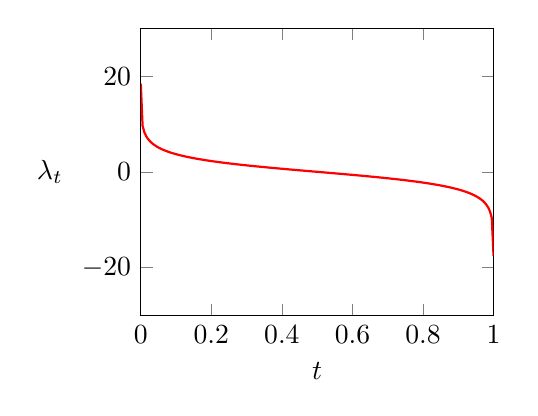
\begin{tikzpicture}
      \begin{axis}[
            xlabel=$t$,
            ylabel=$\lambda_t$,
            ylabel near ticks,
            xlabel near ticks,
            ylabel style={rotate=-90},
            xmin=0,
            xmax=1,
            ymin=-30,
            ymax=30,
            width=.5\linewidth]
      \addplot[color=red,thick,domain=-0.005:1.005,samples=200]{-2 * ln(tan(deg(pi / 2 * ((2 / pi * rad(atan(exp(-0.5 * 30)))) + x * ((2 / pi * rad(atan(exp(-0.5 * -30)))) - (2 / pi * rad(atan(exp(-0.5 * 30)))))))))};
      \end{axis}
      \end{tikzpicture}
      \caption{Relationship between time $t$ and the log signal-to-noise ratio $\lambda_t$ for the truncated continuous-time $\alpha$-cosine noise schedule $f_\Lambda(t)$ as defined in Equation \ref{eq:f_lambda_alpha_cosine} with $\lambda_{\min}=-30$ and $\lambda_{\max}=30$. The horizontal axis is time $t\in[0,1]$; the vertical axis is $\lambda_t=f_\Lambda(t)\in[\lambda_{\min},\lambda_{\max}]=[-30, 30]$.}
      \label{fig:cosine_lambda_t}
\end{figure}
We can compute $\alpha_t$ and $\sigma_t$ from either $\lambda_t$ or $t$ via the following equations:
\begin{alignat}{2}
      \alpha_t&=\sqrt{S(\lambda_t)}&&=\cos\left(\frac{\pi}{2}(t_0+t(t_1-t_0)\right)\label{eq:alpha_t_alpha_cosine}\\
      \sigma_t&=\sqrt{S(-\lambda_t)}&&=\sin\left(\frac{\pi}{2}(t_0+t(t_1-t_0)\right)\label{eq:sigma_t_alpha_cosine}
\end{alignat}
where $S$ is the sigmoid function. Figure \ref{fig:cosine_alpha_sigma} visualises how the values of $\alpha_t$ and $\sigma_t$ vary with time $t\in[0,1]$ using the $\alpha$-cosine schedule detailed above. Appendix \ref{appx:diffusion_cosine_noise_schedule} provides further details on the form of $f_\Lambda$ and how we can derive the forms for $\alpha_t$ and $\sigma_t$.

\begin{figure}[htbp]
      \centering
      \begin{subfigure}{0.49\textwidth}
            \begin{tikzpicture}
            \begin{axis}[
                  xlabel=$t$,
                  ylabel=$\alpha_t$,
                  ylabel near ticks,
                  xlabel near ticks,
                  ylabel style={rotate=-90},
                  xmin=0,
                  xmax=1,
                  ymin=0,
                  ymax=1,
                  width=\linewidth]
            \addplot[color=red,thick,domain=0:1,samples=100]{cos(deg(pi / 2 * ((2 / pi * rad(atan(exp(-0.5 * 30)))) + x * ((2 / pi * rad(atan(exp(-0.5 * -30)))) - (2 / pi * rad(atan(exp(-0.5 * 30))))))))};
            \end{axis}
            \end{tikzpicture}
      \end{subfigure}
      \begin{subfigure}{0.49\textwidth}
            \begin{tikzpicture}
            \begin{axis}[
                  xlabel=$t$,
                  ylabel=$\sigma_t$,
                  ylabel near ticks,
                  xlabel near ticks,
                  ylabel style={rotate=-90},
                  xmin=0,
                  xmax=1,
                  ymin=0,
                  ymax=1,
                  width=\linewidth]
            \addplot[color=red,thick,domain=0:1,samples=100]{sin(deg(pi / 2 * ((2 / pi * rad(atan(exp(-0.5 * 30)))) + x * ((2 / pi * rad(atan(exp(-0.5 * -30)))) - (2 / pi * rad(atan(exp(-0.5 * 30))))))))};
            \end{axis}
            \end{tikzpicture}
      \end{subfigure}
      \caption{Relationship between time $t$ and $\alpha_t$ (left) and $\sigma_t$ (right) for the same truncated continuous-time $\alpha$-cosine noise schedule as that in Figure \ref{fig:cosine_lambda_t}. The horizontal axis is time $t\in[0,1]$; the vertical axis is the value of $\alpha_t$ (left) and $\sigma_t$ (right).}
      \label{fig:cosine_alpha_sigma}
\end{figure}

We can, in theory, use two different noise schedules: one to train the model and another to generate new samples. During training, the noise schedule affects the variance of the gradients \cite{Understanding_Diffusion_Objective_Kingma}. During generation, we typically want to use a noise schedule that optimises the quality of the generated samples. However, in this work, we use the truncated continuous-time $\alpha$-cosine schedule for training and generation, as we found it to provide empirically good results for both. During training, we sampling $t\sim\mathcal{U}(0,1)$ uniformly at random, then compute $\lambda=f_\Lambda(t)$, which equates to sampling $\lambda\sim p_\Lambda(\lambda)$, where $p_\Lambda(\lambda)$ is the probability density function for the truncated continuous-time $\alpha$-cosine schedule, and given by:
\begin{align}
      p_\Lambda(\lambda)=\frac{1}{2\pi(t_1-t_0)}\mathrm{sech}\left(\frac{\lambda}{2}\right)
\end{align}
Figure \ref{fig:p_lambda} displays the probability density function.
\begin{figure}[htbp]
      \centering
      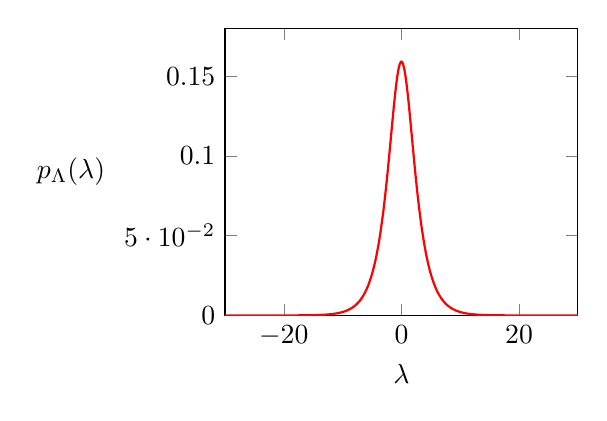
\begin{tikzpicture}
      \begin{axis}[
            xlabel=$\lambda$,
            ylabel=$p_\Lambda(\lambda)$,
            ylabel near ticks,
            xlabel near ticks,
            ylabel style={rotate=-90},
            xmin=-30,
            xmax=30,
            ymin=0,
            ymax=0.18,
            width=.5\linewidth]
      \addplot[color=red,thick,domain=-30:30,samples=300]{ (1 / cosh(x/2)) / (2 * pi * (2 / pi * rad(atan(exp(-0.5 * -30)))) - (2 / pi * rad(atan(exp(-0.5 * 30)))))};
      \end{axis}
      \end{tikzpicture}
      \caption{Probability density function $p_\Lambda(\lambda)$ for the same truncated continuous-time $\alpha$-cosine schedule as that in Figure \ref{fig:cosine_lambda_t}. The horizontal axis is the log signal-to-noise ratio $\lambda\in[\lambda_{\min}, \lambda_{\max}]$; the vertical axis is the corresponding probability density $p_\Lambda$.}
      \label{fig:p_lambda}
\end{figure}

\subsection{Parameterisations}
\label{sec:background_diffusion_parameterisations}

In Section \ref{sec:background_diffusion_reverse}, we defined our generative model $p_\theta(\mathbf{x})$ using $\hat{\mathbf{x}}_\theta(\mathbf{z}_t,\lambda_t)$, which takes as input some noisy latent variable $\mathbf{z}_t$ and a log signal-to-noise ratio $\lambda_t$ and outputs a denoised estimate of the latent. Training a neural network to predict $\mathbf{x}\approx\hat{\mathbf{x}}_\theta(\mathbf{z}_t, \lambda_t)$ directly is referred to as the $\mathbf{x}$-prediction parameterisation, but is seldom adopted in the broader literature due to sub-optimal results \cite{DDPM_Ho}. Recent diffusion models have instead adopted different parameterisations, most commonly the $\boldsymbol\epsilon$-prediction parameterisation (see e.g. \cite{DDPM_Ho,Cascaded_Ho,Imagen_Saharia}), wherein a neural network is instead trained to predict the noise $\boldsymbol\epsilon\approx\hat{\boldsymbol\epsilon}_\theta(\mathbf{z}_t,\lambda_t)$, from which we can compute a denoised estimate of noisy latent $\mathbf{z}_t$ via:
\begin{align}
      \hat{\mathbf{x}}_\theta(\mathbf{z}_t,\lambda_t)=\frac{1}{\alpha_t}\left(\mathbf{z}_t-\sigma_t\hat{\boldsymbol\epsilon}_\theta(\mathbf{z}_t, \lambda_t)\right)
\end{align}
In this work, we employ the $\mathbf{v}$-prediction parameterisation, introduced originally by Salimans and Ho \cite{Progressive_Distillation_Salimans}, and commonly employed in video diffusion models (see e.g. \cite{VDM_Ho,Imagen_Video_Ho}). The $\mathbf{v}$-prediction parameterisation was introduced initially to facilitate progressive distillation for faster sampling, though we utilise it here for its additional benefits highlighted by Ho et al. \cite{Imagen_Video_Ho}, namely faster convergence of sample quality and prevention of temporal colour shifting sometimes observed with $\boldsymbol\epsilon$-prediction video diffusion models. 

Formally, for a given datapoint $\mathbf{x}\sim q(\mathbf{x})$  we define the velocity of $\mathbf{z}_t\sim q(\mathbf{z}_t|\mathbf{x})$ as:
\begin{align}
      \mathbf{v}_t=\alpha_t\boldsymbol\epsilon - \sigma_t\mathbf{x}
\end{align}
where $\boldsymbol\epsilon\sim\mathcal{N}(\mathbf{0}, \mathbf{I})$ is multivariate standard Gaussian noise. We train our neural network $\hat{\mathbf{v}}_\theta(\mathbf{z}_t,\lambda_t)$ to minimise the following loss function, defined per datapoint $\mathbf{x}$ as:
\begin{align}
      \mathbb{E}_{\lambda\sim p_\Lambda(\lambda),\boldsymbol\epsilon\sim\mathcal{N}(\mathbf{0},\mathbf{I})}\left[\Vert\mathbf{v}_t-\hat{\mathbf{v}}_\theta(\mathbf{z}_t, \lambda_t)\Vert_2^2\right]\label{eq:v_parameterisation_loss}
\end{align}
During discrete-time ancestral sampling, we convert our estimate $\mathbf{v}_t\approx\hat{\mathbf{v}}_\theta(\mathbf{z}_t,\lambda_t)$ into an estimate of the denoised latent $\mathbf{x}\approx\hat{\mathbf{x}}_\theta(\mathbf{z}_t,\lambda_t)$ via:
\begin{align}
      \hat{\mathbf{x}}(\mathbf{z}_t,\lambda_t)=\alpha_t\mathbf{z}_t-\sigma_t\hat{\mathbf{v}}_\theta(\mathbf{z}_t,\lambda_t)
\end{align}
Appendix \ref{appx:diffusion_v_prediction_parameterisation} provides further details on the $\mathbf{v}$-prediction parameterisation, including derivations of the velocity and denoised latent.

\subsection{Score-Based Interpretation}

Suppose we have a multivariate Gaussian variable with mean $\boldsymbol\mu$ and covariance $\boldsymbol\Sigma$:
\begin{align}
      \mathbf{z}\sim p(\mathbf{z})=\mathcal{N}(\mathbf{z}; \boldsymbol\mu_{\mathbf{z}}, \boldsymbol\Sigma_{\mathbf{z}})
\end{align}
Tweedie's formula states that:
\begin{align}
\mathbb{E}\left[\boldsymbol\mu_{\mathbf{z}}|\mathbf{z}\right]=\mathbf{z}+\boldsymbol\Sigma_{\mathbf{z}} \nabla_{\mathbf{z}}\log p(\mathbf{z})
\end{align}
As such, for a given latent:
\begin{align}
      \mathbf{z}_t\sim q()
\end{align}
$\mathbf{z}_t\sim\mathcal{N}(\mathbf{z}_t; \alpha_t\mathbf{x}, \sigma_t^2\mathbf{I})$, the expected value of the mean $\boldsymbol{\mu}_{\mathbf{z}_t}$ given $\mathbf{z}_t$ is given by:
\begin{align}
      \mathbb{E}\left[\boldsymbol\mu_{\mathbf{z}_t}|\mathbf{z}_t\right]=\mathbf{z}_t+\sigma_t^2\nabla_{\mathbf{z}_t}\log q(\mathbf{z}_t)
\end{align}
From Equation \ref{eq:q_z_t_given_x}, we have $\boldsymbol\mu_{\mathbf{z}_t}=\alpha_t\mathbf{x}$. Thus, we can reformulate the score of $q(\mathbf{z}_t)$ in terms of $\mathbf{z}_t$ and $\mathbf{x}$ as:
\begin{align}
      \alpha_t\mathbf{x}=\mathbf{z}_t + \sigma_t^2\nabla_{\mathbf{z}_t}\log q(\mathbf{z}_t)
\end{align}


\subsection{ELBO for Diffusion Models}
\label{sec:background_diffusion_elbo}

We can interpret the variance-preserving diffusion model used in this work as an MHVAE with several additional restrictions. Firstly, the dimensionality of each latent $\mathbf{z}_t$ equals the dimensionality of the observed variable. Secondly, we have pre-defined $q(\mathbf{z}_t|\mathbf{z}_s)$ where $0\le s<t\le 1$ as a Gaussian diffusion process with no learnable inference parameters. Finally, the marginal distribution of the final latent $q(\mathbf{z}_1)$ is approximately the multivariate standard Gaussian $\mathcal{N}(\mathbf{0}, \mathbf{I})$, and thus holds effectively no information about the observed variable $\mathbf{x}$. VAEs and MHVAEs do not typically have these restrictions. Nonetheless, much like VAEs and MHVAEs, we can optimise the generative parameters $\theta$ of diffusion models by minimising the ELBO loss. As a notable example, Sohl-Dickstein et al. \cite{Deep_Unsupervised_Learning_Sohl-Dickstein} optimised the original discrete-time diffusion model via the ELBO loss. 

For a given datapoint $\mathbf{x}$, we define $\mathcal{L}_\Lambda(\lambda)$ as the KL divergence of $q(\mathbf{z}_t,\ldots,\mathbf{z}_1|\mathbf{x})$ from $p_\theta(\mathbf{z}_t,\ldots,\mathbf{z}_1)$ for a subset of timesteps from $t=f_\Lambda^{-1}(\lambda)$ to $1$ for datapoint $\mathbf{x}$:
\begin{align}
      \mathcal{L}_\Lambda(\lambda)=D_{KL}(q(\mathbf{z}_t,\ldots,\mathbf{z}_1|\mathbf{x})\Vert p_\theta(\mathbf{z}_t,\ldots,\mathbf{z}_1))
\end{align}
Notably, $\mathcal{L}_\Lambda(\lambda)$ equates to $\mathcal{L}_T(t)$ defined in Equation \ref{eq:dkl_t} under a simple change of variable:
\begin{align}
      \mathcal{L}_\Lambda(\lambda)=\mathcal{L}_T(t=f_\Lambda^{-1}(\lambda))
\end{align}
Similarly, we can reformulate the ELBO loss for a continuous-time MHVAE given in Equation \ref{eq:elbo_mhvae} to provide the ELBO loss in terms of the log signal-to-noise ratio $\lambda$; it is given per datapoint $\mathbf{x}$ by:
\begin{align}
      \mathcal{L}_{\mathrm{ELBO}}(\mathbf{x})&=\mathbb{E}_{\mathbf{z}_0\sim q(\mathbf{z}_0,\mathbf{x})}\left[-\log p_\theta(\mathbf{x}|\mathbf{z}_0)\right]+\mathcal{L}_\Lambda(\lambda_{\max})\\
      &=\underbrace{\mathbb{E}_{\mathbf{z}_0\sim q(\mathbf{z}_0,\mathbf{x})}\left[-\log p_\theta(\mathbf{x}|\mathbf{z}_0)\right]}_{\text{Reconstruction Loss}}+\underbrace{\mathcal{L}_\Lambda(\lambda_{\min})}_{\text{Prior Loss}}+\int_{\lambda_{\min}}^{\lambda_{\max}}\mathcal{L}_\Lambda'(\lambda)d\lambda\label{eq:diffusion_elbo}
\end{align}
With sufficiently large $\lambda_{\max}$, the reconstruction loss is approximately zero since we can almost perfectly reconstruct $\mathbf{x}$ from $\mathbf{z}_0$---this is particularly true for discrete $\mathbf{x}$. Mathematically, as $\lambda_{\max}\to\infty$, we have:
\begin{align}
      \lim_{\lambda_{\max}\to\infty}q(\mathbf{z}_0|\mathbf{x})=\delta(\mathbf{z}_0-\mathbf{x})
\end{align}
where $\delta$ is the Dirac delta distribution. Similarly, with sufficiently small $\lambda_{\min}$, the prior loss is approximately zero; as $\lambda_{\min}\to-\infty$, we have:
\begin{align}
      \lim_{\lambda_{\min}\to -\infty} q(\mathbf{z}_1|\mathbf{x})&=\mathcal{N}(\mathbf{0}, \mathbf{I})=p_\theta(\mathbf{z}_1)
\end{align}
so the KL divergence prior loss term likewise approaches zero.

In Appendix C of \cite{Understanding_Diffusion_Objective_Kingma}, Kingma and Gao showed that $\mathcal{L}_\Lambda'(\lambda)$---which, with a slight abuse of terminology, they refer to as the \textit{time derivative}---simplifies to a remarkable degree:
\begin{align}
      \mathcal{L}_{\Lambda}'(\lambda)=\frac{d}{d\lambda}\mathcal{L}_\Lambda(\lambda)=\frac{1}{2}\mathbb{E}_{\boldsymbol\epsilon\sim\mathcal{N}(\mathbf{0}, \mathbf{I})}\left[\Vert \boldsymbol\epsilon -\hat{\boldsymbol\epsilon}_\theta(\mathbf{z}_t,\lambda_t)\Vert_2^2\right]\label{eq:time_derivative}
\end{align} 

\subsection{Weighted Loss}
\label{sec:background_diffusion_weighted_loss}

Most diffusion models in the broader literature---including state-of-the-art models---do not optimise their parameters $\theta$ via minimisation of the ELBO loss. In practice, the various objectives used are all special cases of a \textit{weighted loss} \cite{Understanding_Diffusion_Objective_Kingma}, which is defined per datapoint $\mathbf{x}$ as:
\begin{align}
      \mathcal{L}_{\mathrm{WL}}&=w(\lambda_{\min})\mathcal{L}_\Lambda(\lambda_{\min})+\int_{\lambda_{\min}}^{\lambda_{\max}}w(\lambda)\mathcal{L}_\Lambda'(\lambda)d\lambda
\end{align}
where $w(\lambda)$ is a weighting function. Note that, assuming the reconstruction loss is approximately zero, the ELBO loss given in Equation \ref{eq:diffusion_elbo} is a special case of the weighted loss $\mathcal{L}_{\mathrm{WL}}$ with $w(\lambda) = 1$. Substituting the form of $\mathcal{L}'_\Lambda(\lambda)$ given in Equation \ref{eq:time_derivative} yields the following form for the weighted loss:
\begin{align}
      \mathcal{L}_{\mathrm{WL}}&=w(\lambda_{\min})\mathcal{L}_\Lambda(\lambda_{\min})+\frac{1}{2}\int_{\lambda_{\min}}^{\lambda_{\max}}w(\lambda)\mathbb{E}_{\boldsymbol\epsilon\sim\mathcal{N}(\mathbf{0},\mathbf{I})}\left[\Vert\boldsymbol\epsilon-\hat{\boldsymbol\epsilon}_\theta(\mathbf{z}_t,\lambda)\Vert_2^2\right]d\lambda
\end{align}
This form provides several useful insights. Since the first term---the weighted prior loss---contains no learnable parameters, minimisation of the weighted loss $\mathcal{L}_{\mathrm{WL}}$ equates to minimisation of the intractable integral. In practice, we minimise the integral via an importance-weighted Monte Carlo integrator:
\begin{align}
      \int_{\lambda_{\min}}^{\lambda_{\max}}w(\lambda)\mathbb{E}_{\boldsymbol\epsilon\sim\mathcal{N}(\mathbf{0},\mathbf{I})}\left[\Vert\boldsymbol\epsilon-\hat{\boldsymbol\epsilon}_\theta(\mathbf{z}_t,\lambda_t)\Vert_2^2\right]d\lambda&=\mathbb{E}_{\lambda\sim p_\Lambda(\lambda)}\left[\frac{w(\lambda)}{p_\Lambda(\lambda)}\mathbb{E}_{\boldsymbol\epsilon\sim\mathcal{N}(\mathbf{0},\mathbf{I})}\left[\Vert\boldsymbol\epsilon - \hat{\boldsymbol\epsilon}_\theta(\mathbf{z}_t, \lambda)\Vert_2^2 \right]\right]\\
      &=\mathbb{E}_{\lambda\sim p_\Lambda(\lambda),\boldsymbol\epsilon\sim\mathcal{N}(\mathbf{0}, \mathbf{I})}\left[\frac{w(\lambda)}{p_\Lambda(\lambda)}\Vert \boldsymbol\epsilon-\hat{\boldsymbol\epsilon}_\theta(\mathbf{z}_t,\lambda)\Vert_2^2\right]\\
      &\simeq \frac{w(\lambda)}{p_\Lambda(\lambda)}\Vert \boldsymbol\epsilon-\hat{\boldsymbol\epsilon}_\theta(\mathbf{z}_t,\lambda)\Vert_2^2
\end{align}
Notable further analysis by Kingma and Gao \cite{Understanding_Diffusion_Objective_Kingma} shows that the weighted loss also has a likelihood-based interpretation. Simple integration by parts enables us to write the weighted loss as:
\begin{align}
      \mathcal{L}_{\mathrm{WL}} = w(\lambda_{\max})\mathcal{L}_\Lambda(\lambda_{\max}) + \int_{\lambda_{\min}}^{\lambda_{\max}}-w'(\lambda)\mathcal{L}_\Lambda(\lambda) d\lambda
\end{align}
The likelihood-based interpretation comes from the fact that $\mathcal{L}_\Lambda(\lambda)$ serves as a variational bound on the negative marginal likelihood of the noise-perturbed data $\mathbf{z}_t\sim q(\mathbf{z}_t|\mathbf{x})$:
\begin{align}
      \mathcal{L}_\Lambda(\lambda)&\ge D_{KL}(q(\mathbf{z}_t|\mathbf{x})\Vert p(\mathbf{z}_t))\\
      &=\mathbb{E}_{\mathbf{z}_t\sim q(\mathbf{z}_t|\mathbf{x})}\left[-\log p(\mathbf{z}_t)\right]+\mathbb{E}_{\mathbf{z}_t\sim q(\mathbf{z}_t|\mathbf{x})}\left[\log q(\mathbf{z}_t|\mathbf{x})\right]
\end{align}
As such, minimisation of $\mathcal{L}_\Lambda(\lambda)$ equates to maximisation of the expected log-likelihood of the noise-perturbed data $\mathbf{z}_t\sim q(\mathbf{z}_t|\mathbf{x})$ with noise level $\lambda$. If the weighting function $w(\lambda)$ is a monotonically decreasing function of $\lambda\in [\lambda_{\min}, \lambda_{\max}]$, then by definition $-w'(\lambda)$ will be positive for all $\lambda\in [\lambda_{\min}, \lambda_{\max}]$. In which case, minimisation of $\mathcal{L}_{\mathrm{WL}}$ itself equates to maximisation of the weighted expected log-likelihood of the noise-perturbed data $\mathbf{z}_t\sim q(\mathbf{z}_t|\mathbf{x})$ with weighting $-w'(\lambda)$. 

Kingma and Gao's \cite{Understanding_Diffusion_Objective_Kingma} analysis directly justifies our use of the $\mathbf{v}$-prediction parameterisation with the truncated continuous-time $\alpha$-cosine noise schedule. In conjunction, their use equates to the weighted loss with:
\begin{align}
      w(\lambda)&=\frac{1}{2\pi(t_1-t_0)}\exp\left(-\frac{\lambda}{2}\right)\\
      -w'(\lambda)&=\frac{1}{4\pi(t_1-t_0)}\exp\left(-\frac{\lambda}{2}\right)
\end{align}
Figure \ref{fig:v_prediction_weighting} shows the weighting function $w(\lambda)$ and the negative of its derivative $-w'(\lambda)$ for the $\mathbf{v}$-parameterisation loss. As evident from the graphs, the weighting function $w(\lambda)$ is a monotonically decreasing function of $\lambda$, and as such $-w'(\lambda)$ is positive for all $\lambda\in [\lambda_{\min}, \lambda_{\max}]$. Therefore, during training, we are maximising a weighted expected log-likelihood of noise-perturbed data $\mathbf{z}_t\sim q(\mathbf{z}_t|\mathbf{x})$ for all $\lambda\in[\lambda_{\min}, \lambda_{\max}]$. In contrast, most diffusion models in the broader literature (see e.g. \cite{DDPM_Ho,IDDPM_Nichol,Imagen_Saharia}) undergo training with non-monotonic weighting functions. In such cases, for noise levels whereby $-w'(\lambda)$ is negative, the weighted loss has a counterintuitive interpretation of minimisation of the weighted expected log-likelihood of the noise-perturbed data $\mathbf{z}_t\sim q(\mathbf{z}_t|\mathbf{x})$.
\begin{figure}[htbp]
      \centering
      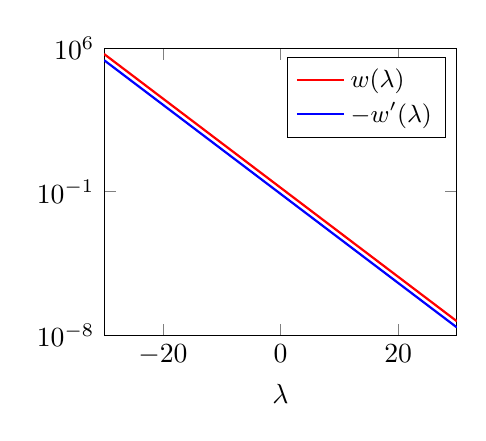
\begin{tikzpicture}
            \begin{axis}[
                  xlabel=$\lambda$,
                  ymode = log,
                  xmin=-30,
                  xmax=30,
                  ymin=0.00000001,
                  ymax=1000000,
                  width=.5\linewidth,
                  legend pos=north east,
                  legend style={font=\small},
                  legend cell align={left},
                  ylabel style={rotate=-90},
                  ylabel near ticks,
                  xlabel near ticks
                  ]
                  \addplot[color=red,thick,domain=-30:30,samples=100]{1 / ((2 * pi * (2 / pi * rad(atan(exp(-0.5 * -30)))) - (2 / pi * rad(atan(exp(-0.5 * 30)))))) * exp(-x / 2)};
                  \addlegendentry{$w(\lambda)$}
                  \addplot[color=blue,thick,domain=-30:30,samples=100]{1 / ((4 * pi * (2 / pi * rad(atan(exp(-0.5 * -30)))) - (2 / pi * rad(atan(exp(-0.5 * 30)))))) * exp(-x / 2)};
                  \addlegendentry{$-w'(\lambda)$}
                  \end{axis}
      \end{tikzpicture}
      \caption{Relationship between the log signal-to-noise ratio $\lambda$ and the functions $w(\lambda)$ and $-w'(\lambda)$ for the $\mathbf{v}$-parameterisation with the same truncated continuous-time $\alpha$-cosine schedule as that in Figure \ref{fig:cosine_lambda_t}. The horizontal axis is the log signal-to-noise level $\lambda$; the vertical axis is the value of $w(\lambda)$ and $-w'(\lambda)$; the vertical axis is logarithmic.}
      \label{fig:v_prediction_weighting}
\end{figure}

\subsection{Imputation for Conditional Generation}

In Section \ref{sec:background_conditional}, we introduced the concept of conditional generation. In this work, however, we do not train a conditional model explicitly. Instead, we utilise \textit{reconstruction-guided sampling} \cite{VDM_Ho}: a sophisticated technique that derives a conditional model approximately from an unconditional model. More specifically, reconstruction-guided sampling facilitates the conditional generation of the unknown dimensions of some observed datapoint $\mathbf{x}$ given the known dimensions. Deriving such a conditional model approximately from an unconditional model is advantageous: it enables us to train only a single unconditional model, which we can then flexibly use to facilitate the conditional generation of any unknown subset of dimensions.  In this work, we utilise reconstruction-guided sampling to facilitate three distinct conditional generation tasks: temporal interpolation, forecasting, and autoregressive generation of arbitrarily long samples. 

Reconstruction-guided sampling extends a prior technique known as \textit{imputation}, introduced by Song et al. \cite{Score_Based_Song}. Thus, we first introduce imputation for completeness and to better motivate our use of reconstruction-guided sampling in this work.

We denote by $\Omega(\mathbf{x})$ and $\bar\Omega(\mathbf{x})$ the known and unknown dimensions of some observed datapoint $\mathbf{x}$, respectively. Formally, our goal is to derive the following conditional model without training it explicitly:
\begin{align}
      p_\theta(\bar\Omega(\mathbf{x})|\Omega(\mathbf{x}))
\end{align}
We can write the forward diffusion process for the unknown dimensions as the following SDE:
\begin{align}
      d\bar\Omega(\mathbf{z}_t)=\mathbf{f}(\bar\Omega(\mathbf{z}_t), t) + g(t)d\mathbf{w}_t
\end{align}
Anderson \cite{Reverse_Time_Diffusion_Anderson} shows that the corresponding reverse-time SDE conditioned on the known dimensions $\Omega(\mathbf{x})$ is given by:
\begin{align}
      d\bar\Omega(\mathbf{z}_t)=\left[\mathbf{f}(\bar\Omega(\mathbf{z}_t), t) - g(t)^2\nabla_{\bar\Omega(\mathbf{z}_t)}\log q(\bar\Omega(\mathbf{z}_t)|\Omega(\mathbf{x}))\right]dt + g(t)d \bar{\mathbf{w}}_t\label{eq:recon_reverse_sde}
\end{align}
Although $q(\bar\Omega(\mathbf{z}_t)|\Omega(\mathbf{x}))$ is intractable, we can approximate it as follows:
\begin{align}
      q(\bar\Omega(\mathbf{z}_t)|\Omega(\mathbf{x}))&=\int q(\bar\Omega(\mathbf{z}_t), \Omega(\mathbf{z}_t)|\Omega(\mathbf{x}))d\Omega(\mathbf{z}_t)\\
      &=\int q(\bar\Omega(\mathbf{z}_t)|\Omega(\mathbf{x}), \Omega(\mathbf{z}_t))q(\Omega(\mathbf{z}_t)|\Omega(\mathbf{x})) d\Omega(\mathbf{z}_t)\\
      &=\mathbb{E}_{\Omega(\mathbf{z}_t)\sim q(\Omega(\mathbf{z}_t)|\Omega(\mathbf{x}))}\left[q(\bar\Omega(\mathbf{z}_t)|\Omega(\mathbf{x}), \Omega(\mathbf{z}_t))\right]\\
      &\approx \mathbb{E}_{\Omega(\mathbf{z}_t)\sim q(\Omega(\mathbf{z}_t)|\Omega(\mathbf{x}))}\left[q(\bar\Omega(\mathbf{z}_t)| \Omega(\mathbf{z}_t))\right]\label{eq:imputation_assumption}
\end{align}
Song et al. \cite{Score_Based_Song} argue that the approximation in Equation \ref{eq:imputation_assumption} is appropriate since for small $t$, $\Omega(\mathbf{x})$ is almost the same as $\Omega(\mathbf{z}_t)$; and for larger $t$, $\Omega(\mathbf{x})$ is further away from $\bar\Omega(\mathbf{z}_t)$ in the Markov chain, and thus has a smaller impact on $\bar\Omega(\mathbf{z}_t)$. Assuming the approximation holds, we can derive an unbiased estimator of $q(\bar\Omega(\mathbf{z}_t)|\Omega(\mathbf{x}))$ as:
\begin{align}
      q(\bar\Omega(\mathbf{z}_t)|\Omega(\mathbf{x})) \approx \mathbb{E}_{\Omega(\mathbf{z}_t)\sim q(\Omega(\mathbf{z}_t)|\Omega(\mathbf{x}))}\left[q(\bar\Omega(\mathbf{z}_t)| \Omega(\mathbf{z}_t))\right] \simeq q(\bar\Omega(\mathbf{z}_t)| \Omega(\mathbf{z}_t))
\end{align}
The score of the natural logarithm of the unbiased estimator is given by:
\begin{align}
      \nabla_{\bar\Omega(\mathbf{z}_t)} \log q(\bar\Omega(\mathbf{z}_t)| \Omega(\mathbf{z}_t))&=\nabla_{\bar\Omega(\mathbf{z}_t)} \log q(\bar\Omega(\mathbf{z}_t), \Omega(\mathbf{z}_t)) - \nabla_{\bar\Omega(\mathbf{z}_t)} \log q(\Omega(\mathbf{z}_t))\\
      &=\nabla_{\bar\Omega(\mathbf{z}_t)} \log q(\bar\Omega(\mathbf{z}_t), \Omega(\mathbf{z}_t))\\
      &=\nabla_{\bar\Omega(\mathbf{z}_t)} \log q([\bar\Omega(\mathbf{z}_t); \Omega(\mathbf{z}_t)])
\end{align}
where $[\bar\Omega(\mathbf{z}_t); \Omega(\mathbf{z}_t)]$ denotes a vector such that:
\begin{align}
      \Omega([\bar\Omega(\mathbf{z}_t); \Omega(\mathbf{z}_t)]) = \Omega(\mathbf{z}_t)\\
      \bar\Omega([\bar\Omega(\mathbf{z}_t); \Omega(\mathbf{z}_t)]) = \bar\Omega(\mathbf{z}_t)
\end{align}
Thus, assuming the assumption given in Equation \ref{eq:imputation_assumption} holds, we can consequently approximate the reverse-time SDE conditioned on $\Omega(\mathbf{x})$ given in Equation \ref{eq:recon_reverse_sde} as follows:
\begin{align}
      d\bar\Omega(\mathbf{z}_t)=\left[\mathbf{f}(\bar\Omega(\mathbf{z}_t), t) - g(t)^2\nabla_{\bar\Omega(\mathbf{z}_t)}\log q([\bar\Omega(\mathbf{z}_t); \Omega(\mathbf{z}_t)])\right]dt + g(t)d \bar{\mathbf{w}}_t
\end{align}
If we have a perfect score model, $\mathbf{s}_\theta(\mathbf{z}_t, \lambda_t)=\nabla_{\mathbf{z}_t} q(\mathbf{z}_t)$, then the reverse-time SDE is thus given by:
\begin{align}
      d\bar\Omega(\mathbf{z}_t)=\left[\mathbf{f}(\bar\Omega(\mathbf{z}_t), t) - g(t)^2 \mathbf{s}_\theta([\bar\Omega(\mathbf{z}_t); \Omega(\mathbf{z}_t)], \lambda_t)\right]dt + g(t)d \bar{\mathbf{w}}_t\label{eq:imputation_reverse_sde}
\end{align}
To provide a more intuitive link between Equation \ref{eq:imputation_reverse_sde} and the generative procedure in Section \ref{sec:background_climate_generative}, we also define the imputation method as a conditional denoiser $\hat{\mathbf{x}}^{\mathrm{C}}_\theta(\mathbf{z}_t, \lambda_t, \Omega(\mathbf{x}))$, which takes the known dimensions of $\mathbf{x}$ as input:
\begin{align}
      \hat{\mathbf{x}}^{\mathrm{C}}_\theta(\mathbf{z}_t, \lambda_t, \Omega(\mathbf{x}))=\bar\Omega\left(\hat{\mathbf{x}}_\theta([\bar\Omega(\mathbf{z}_t); \Omega(\mathbf{z}_t)], \lambda_t )\right)
\end{align}
Thus, the imputation method for conditional generation yields only a slight adjustment to the generative procedure defined in Section \ref{sec:background_diffusion_reverse}. Namely, at each step of the discrete-time ancestral sampler, we replace the dimensions of $\mathbf{z}_t$ corresponding to the known dimensions of $\mathbf{x}$ with an exact sample from the forward process: $\Omega(\mathbf{z}_t)\sim q(\Omega(\mathbf{z}_t)|\Omega(\mathbf{x}))$.

\subsection{Reconstruction-Guided Sampling for Conditional Generation}
\label{sec:background_diffusion_reconstruction_guided_sampling}

Ho et al. \cite{VDM_Ho} showed that the imputation process produces incoherent samples when applied to video diffusion models. Namely, although a given $\bar\Omega(\mathbf{x})$ will often appear reasonable in isolation, it will often not be coherent with $\Omega(\mathbf{x})$. This incoherency is likely because the assumption in Equation \ref{eq:imputation_assumption} does not hold for all $t\in[0,1]$. Avoiding the assumption, we instead construct an unbiased estimator for $q(\bar\Omega(\mathbf{z}_t|\Omega(\mathbf{x})))$ as:
\begin{align}
      q(\bar\Omega(\mathbf{z}_t)|\Omega(\mathbf{x}))&=\mathbb{E}_{\Omega(\mathbf{z}_t)\sim q(\Omega(\mathbf{z}_t)|\Omega(\mathbf{x}))}\left[q(\bar\Omega(\mathbf{z}_t)|\Omega(\mathbf{x}), \Omega(\mathbf{z}_t))\right] \simeq q(\bar\Omega(\mathbf{z}_t)|\Omega(\mathbf{x}), \Omega(\mathbf{z}_t))
\end{align}
The score of the natural logarithm of the unbiased estimator is given by:
\begin{align}
      \nabla_{\bar\Omega(\mathbf{z}_t)} \log q(\bar\Omega(\mathbf{z}_t)|\Omega(\mathbf{x}),\Omega(\mathbf{z}_t))&=\nabla_{\bar\Omega(\mathbf{z}_t)} \log q(\bar\Omega(\mathbf{z}_t), \Omega(\mathbf{x}), \Omega(\mathbf{z}_t))-\nabla_{\bar\Omega(\mathbf{z}_t)}\log q(\Omega(\mathbf{z}_t),\Omega(\mathbf{x}))\\
      &=\nabla_{\bar\Omega(\mathbf{z}_t)} \log q(\bar\Omega(\mathbf{z}_t), \Omega(\mathbf{x}), \Omega(\mathbf{z}_t))\\
      &=\nabla_{\bar\Omega(\mathbf{z}_t)} \log q(\bar\Omega(\mathbf{z}_t), \Omega(\mathbf{z}_t)) + \nabla_{\bar\Omega(\mathbf{z}_t)} \log q(\Omega(\mathbf{x})|\bar\Omega(\mathbf{z}_t), \Omega(\mathbf{z}_t))\\
      &=\nabla_{\bar\Omega(\mathbf{z}_t)} \log q([\bar\Omega(\mathbf{z}_t); \Omega(\mathbf{z}_t)]) + \nabla_{\bar\Omega(\mathbf{z}_t)} \log q(\Omega(\mathbf{x})|[\bar\Omega(\mathbf{z}_t); \Omega(\mathbf{z}_t)])\label{eq:recon_reverse_sde_score}
\end{align}
The second term in Equation \ref{eq:recon_reverse_sde_score} is missing in the imputation approach. Plugging in this missing term would make conditional sampling exact. However, since $q(\Omega(\mathbf{x})|[\bar\Omega(\mathbf{z}_t); \Omega(\mathbf{z}_t)])$ is not available in closed form, we must approximate it. Ho et al. \cite{VDM_Ho} proposed to approximate it with a multivariate Gaussian of the form:
\begin{align}
      q(\Omega(\mathbf{x})|[\bar\Omega(\mathbf{z}_t); \Omega(\mathbf{z}_t)]) \approx \mathcal{N}\left(\Omega(\mathbf{x}); \Omega\left(\hat{\mathbf{x}}_\theta\left([\bar\Omega(\mathbf{z}_t); \Omega(\mathbf{z}_t)], \lambda_t \right)\right), \left(\frac{\sigma_t^2}{\alpha_t^2}\right)\mathbf{I}\right)
\end{align}
Under this approximation, the second term of Equation \ref{eq:recon_reverse_sde_score} is thus itself approximated by:
\begin{align}
      \nabla_{\bar\Omega(\mathbf{z}_t)} \log q(\Omega(\mathbf{x})|[\bar\Omega(\mathbf{z}_t); \Omega(\mathbf{z}_t)])\approx-\frac{\alpha_t^2}{2\sigma_t^2}\nabla_{\bar\Omega(\mathbf{z}_t)} \left\Vert \Omega(\mathbf{x}) - \Omega\left(\hat{\mathbf{x}}_\theta\left([\bar\Omega(\mathbf{z}_t); \Omega(\mathbf{z}_t)], \lambda_t \right)\right)\right\Vert_2^2
\end{align}
Ho et al. \cite{VDM_Ho} interpret the inclusion of this term---absent in the imputation method---as a form of \textit{guidance} based on the model's reconstruction of the conditioning data. They found empirically that---as with other forms of guidance---including a large weighting term $w_r>1$ tends to improve sample quality further. They refer to this technique as \textit{reconstruction-guided sampling}. Formally, assuming we have a perfect score model $\mathbf{s}_\theta(\mathbf{z}_t, \lambda_t)=\nabla_{\mathbf{z}_t} q(\mathbf{z}_t)$, reconstruction-guided sampling derives a conditional model from an unconditional model by approximating the score given in Equation \ref{eq:recon_reverse_sde} by:
\begin{align}
      \nabla_{\bar\Omega(\mathbf{z}_t)}\log q(\bar\Omega(\mathbf{z}_t)|\Omega(\mathbf{x}))&\approx \mathbf{s}_\theta ([\bar\Omega(\mathbf{z}_t); \Omega(\mathbf{z}_t)], \lambda_t)\\&-\frac{w_r\alpha_t^2}{2\sigma_t^2}\nabla_{\bar\Omega(\mathbf{z}_t)} \left\Vert \Omega(\mathbf{x}) - \Omega\left(\hat{\mathbf{x}}_\theta\left([\bar\Omega(\mathbf{z}_t); \Omega(\mathbf{z}_t)], \lambda_t \right)\right)\right\Vert_2^2
\end{align}
Writing the reconstruction-guidance method as a conditional denoiser $\hat{\mathbf{x}}^{\mathrm{C}}_\theta(\mathbf{z}_t, \lambda_t, \Omega(\mathbf{x}))$ yields:
\begin{align}
      \hat{\mathbf{x}}^{\mathrm{C}}_\theta(\mathbf{z}_t, \lambda_t, \Omega(\mathbf{x}))=\bar\Omega\left(\hat{\mathbf{x}}_\theta([\bar\Omega(\mathbf{z}_t); \Omega(\mathbf{z}_t)], \lambda_t )\right) - \frac{w_r\alpha_t}{2}\nabla_{\bar\Omega(\mathbf{z}_t)} \left\Vert \Omega(\mathbf{x}) - \Omega\left(\hat{\mathbf{x}}_\theta\left([\bar\Omega(\mathbf{z}_t); \Omega(\mathbf{z}_t)]\right)\right)\right\Vert_2^2
\end{align}

\subsection{U-Net}
\label{sec:background_unet}



\chapter{Climate Background}
\label{chap:background_climate}

\section{Climate Simulations}
\label{sec:background_climate_simulations}

\section{Generative Models for Climate Simulations}
\label{sec:background_climate_generative}

% -----------------------------------------------------------------------------

\chapter{Results}
\label{chap:results}

\section{Dataset}
\label{sec:results_dataset}

\subsection{UKCP18}
\label{sec:results_dataset_ukcp18}

\subsection{Train and Test Sets}
\label{sec:results_dataset_train_test}

We scale each input data element to the range $[-1,1]$ to ensure that our neural network operates on consistently scaled inputs during the reverse-time generative process, starting from the multivariate standard Gaussian prior.

\section{Importance of the Transformation}
\label{sec:results_importance_of_transformation}

\subsection{No Transformation}
\label{sec:results_no_transformation}

One of the primary contributions of this work is a demonstration that the transformation of the input data is critical to the model's performance. To motivate this, we first provide results for a model trained without transforming the input data. Notably, the model produced samples with significant noise at the lower end of the precipitation scale. Figure \ref{fig:no_transform_sample} depicts an example of this. 

\begin{figure}[htbp]
      \centering
      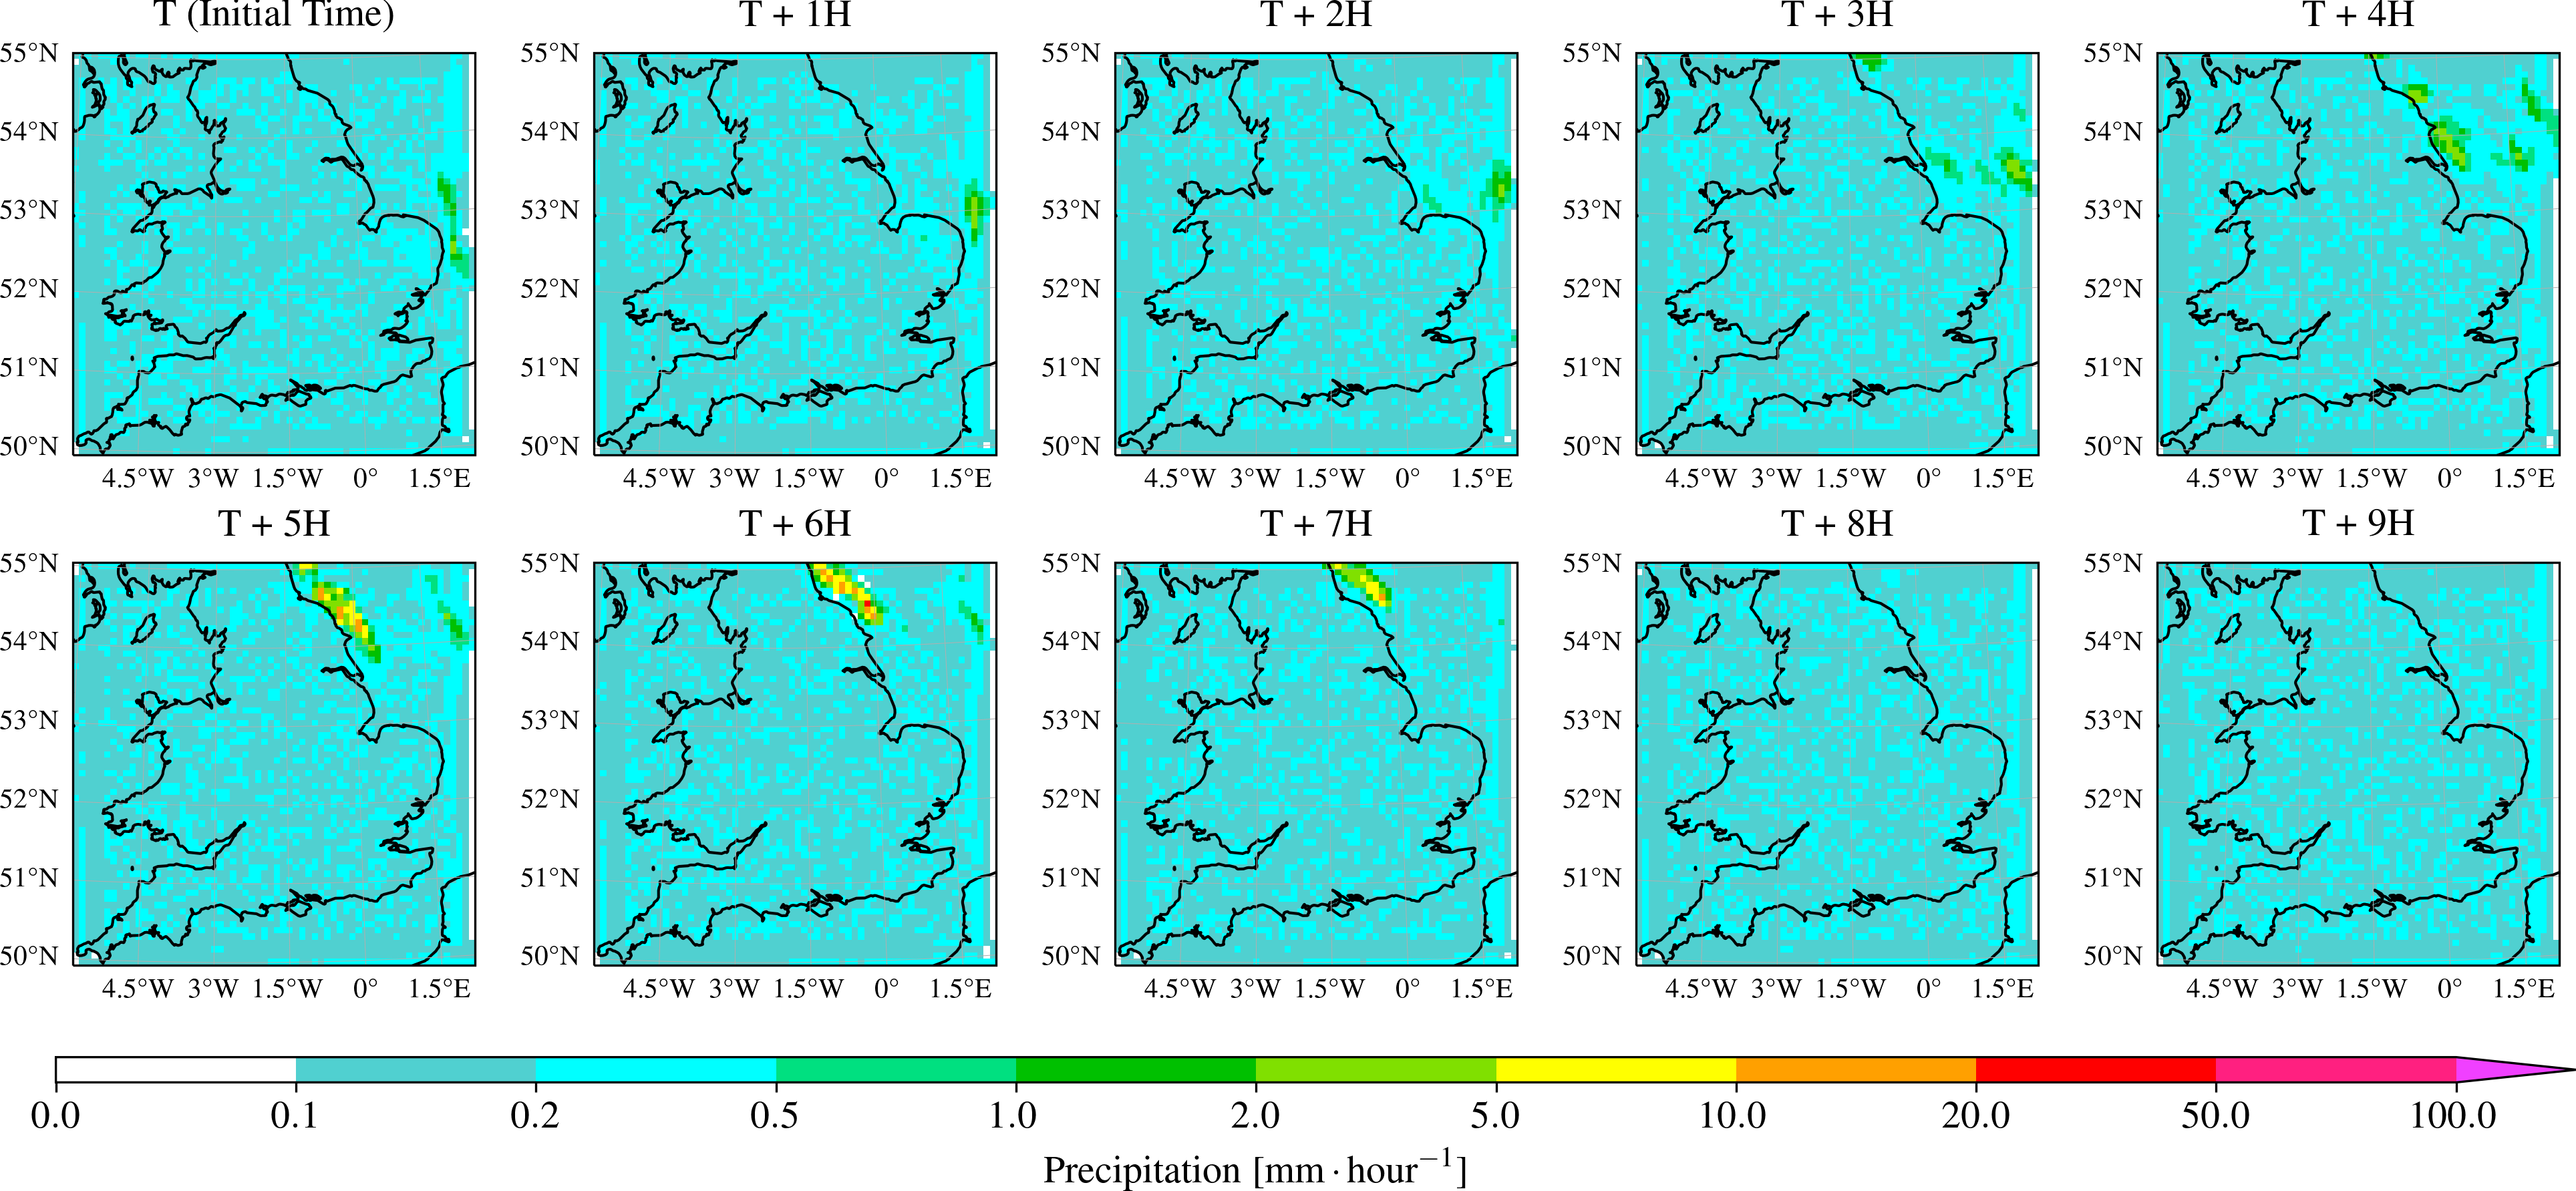
\includegraphics[width=\linewidth]{no_transform_noisy.png}
      \caption{Randomly selected sample generated via our model trained with no transformation of the input data. The sample depicts hourly precipitation for the same $563.2\ \mathrm{km} \times 563.2\ \mathrm{km}$ region centred on Birmingham, UK, over ten hours. Each grid cell illustrates the mean precipitation rate, measured in millimetres per hour, for an $8.8 \ \mathrm{km} \times 8.8\ \mathrm{km}$ subarea.}
      \label{fig:no_transform_sample}
\end{figure}

\subsection{Square Root Transformation}

\subsection{Change of Variable Rule}
\label{sec:results_change_of_variable}

Suppose we transform our observed variable $\mathbf{x}$ via an element-wise monotonically-increasing vector-valued function $\mathbf{h}:[0, \mathrm{P}_{\max}]^D\to[-1,1]^D$, such that:
\begin{align}
      \mathbf{h}(\mathbf{x})=
      \begin{bmatrix}
            h(x_1) \\
            h(x_2) \\
            \vdots \\
            h(x_D)
      \end{bmatrix}
\end{align}
where we select $\mathrm{P}_{\max}$ as the maximum precipitation rate observed in the training set. In other words, our vector-valued function $\mathbf{h}$ applies an identical transformation $h:[0, \mathrm{P}_{\max}]\to[-1,1]$ to each element $x_i$ of $\mathbf{x}$. The change of variable rule states that:
\begin{align}
      p_\theta(\mathbf{x}) = \tilde{p}_\theta(\mathbf{h}(\mathbf{x}))\left|\det\left(\frac{d \mathbf{h}(\mathbf{x})}{d \mathbf{x}}\right)\right|
\end{align}
where $\det$ is the determinant operator, and $d\mathbf{h}(\mathbf{x})/d\mathbf{x}$ is the Jacobian of transformation $\mathbf{h}$. Since $\mathbf{h}$ is an element-wise transformation, the Jacobian matrix is diagonal:
\begin{align}
      \frac{d\mathbf{h}(\mathbf{x})}{d\mathbf{x}} =
      \begin{bmatrix}
            \frac{\partial \tilde{x}_1}{\partial x_1} & 0 & \cdots & 0 \\
            0 & \frac{\partial \tilde{x}_2}{\partial x_2} & \cdots & 0 \\
            \vdots & \vdots & \ddots & \vdots \\
            0 & 0 & \cdots & \frac{\partial \tilde{x}_D}{\partial x_D}
      \end{bmatrix}
\end{align}
The determinant of a diagonal matrix is simply the product of its diagonal elements; thus, we can write:
\begin{align}
      \det\left(\frac{d\mathbf{h}(\mathbf{x})}{d\mathbf{x}}\right) = \prod_{i=1}^D \frac{\partial h(x_i)}{\partial x_i}.
\end{align}
Therefore, we can rewrite the change of variables rule under transformation $\mathbf{h}$ in the following simplified form:
\begin{align}
      p_\theta(\mathbf{x}) = \tilde{p}_\theta(\mathbf{h}(\mathbf{x}))\prod_{i=1}^D \frac{\partial h(x_i)}{\partial x_i}
\end{align}
We can thus formulate the negative log-likelihood of $\mathbf{x}$ as follows:
\begin{align}
      -\log p_\theta(\mathbf{x}) &= -\log \left(\tilde{p}_\theta(\mathbf{h}(\mathbf{x}))\prod_{i=1}^D\frac{\partial h(x_i)}{\partial x_i}\right)\\
      &= -\log \tilde{p}_\theta(\mathbf{h}(\mathbf{x})) - \log\left(\prod_{i=1}^D\frac{\partial h(x_i)}{\partial x_i}\right)\\
      &= -\log \tilde{p}_\theta(\mathbf{h}(\mathbf{x})) - \sum_{i=1}^D \log \left(\frac{\partial h(x_i)}{\partial x_i}\right)\label{eq:minus_log_in_terms_of_minus_log_transform}
\end{align}

\subsection{ELBO Loss with a Change of Variable}
\label{sec:results_elbo_change_of_variable}

The ELBO loss for a transformed datapoint $\mathbf{h}(\mathbf{x})$, denoted $\tilde{\mathcal{L}}_{\mathrm{ELBO}}(\mathbf{h}(\mathbf{x}))$, serves as a variational bound on the negative log-likelihood of $\mathbf{h}(\mathbf{x})$ and is given by:
\begin{align}
      -\log \tilde{p}_\theta(\mathbf{h}(\mathbf{x}))\le \tilde{\mathcal{L}}_{\mathrm{ELBO}}(\mathbf{h}(\mathbf{x})) = \mathbb{E}_{\mathbf{z}_0,\ldots,\mathbf{z}_1\sim\tilde{q}(\mathbf{z}_0,\ldots,\mathbf{z}_1|\mathbf{h}(\mathbf{x}))} \left[\log \frac{\tilde{p}_\theta(\mathbf{z}_0,\ldots,\mathbf{z}_1,\mathbf{h}(\mathbf{x}))}{\tilde{q}(\mathbf{z}_0,\ldots,\mathbf{z}_1|\mathbf{h}(\mathbf{x}))}\right]
\end{align}
Plugging the inequality into Equation \ref{eq:minus_log_in_terms_of_minus_log_transform}, we obtain:
\begin{align}
      -\log p_\theta(\mathbf{x})\le \tilde{\mathcal{L}}_{\mathrm{ELBO}}(\mathbf{h}(\mathbf{x})) - \sum_{i=1}^D \log \left(\frac{\partial h(x_i)}{\partial x_i}\right)\label{eq:optimal_elbo_no_parameters}
\end{align}
Thus, if we were to parameterise the transformation $\mathbf{h}_\omega$, with transformative parameters $\omega$, we would theoretically be able to learn some optimal transformation to approximately minimise the negative log-likelihood of the observed variable $\mathbf{x}$. For completeness, the loss with transformative parameters $\omega$ yields only a minor modification to Equation \ref{eq:optimal_elbo_no_parameters} and is given by:
\begin{align}
      p_\theta(\mathbf{x}) \le \tilde{\mathcal{L}}_{\mathrm{ELBO}}(\mathbf{h}(\mathbf{x})) - \sum_{i=1}^D \log \left(\frac{\partial h_\omega(x_i)}{\partial x_i}\right)\label{eq:optimal_elbo_parameters}
\end{align}
However, as detailed in Section \ref{sec:background_diffusion_weighted_loss}, optimising our generative parameters $\theta$ via the ELBO loss yields suboptimal results. Diffusion models in the broader literature have achieved far superior results via optimisation with the weighted loss $\mathcal{L}_{\mathrm{WL}}$.

\subsection{Weighted Loss with a Change of Variable}

The $\lambda$-dependent weighting function $w(\lambda)$ in the weighted loss $\mathcal{L}_{\mathrm{WL}}$ causes it to lose a direct theoretical relationship with the negative log-likelihood of the observed variable $\mathbf{x}$. Thus, we cannot directly apply the change of variable approach to the weighted loss as we did for the ELBO loss. However, we can consider the individual contribution of the negative log-determinant term in the loss given in Equation \ref{eq:optimal_elbo_parameters} to derive an empirically good loss function for our diffusion model that jointly optimises the generative parameters $\theta$ and the transformative parameters $\omega$. Importantly, since we constrain the output range of $h_\omega$ to be $[-1,1]$, the neural network cannot infinitely extend the output range. As such, it has to learn some optimal monotonically increasing function to minimise:
\begin{align}
      -\sum_{i=1}^D \log \left(\frac{\partial h_\omega(x_i)}{\partial x_i}\right)
\end{align}
Intuitively, since the $\log$ function itself is monotonically increasing, the negative log-determinant term will encourage a steeper gradient for areas of the input space $[0, \mathrm{P}_{\max}]$ wherein individual elements $x_i$ occur most often. Conversely, the term will individually encourage a shallower gradient for areas of the input space $[0, \mathrm{P}_{\max}]$ wherein individual elements $x_i$ occur least often.

Using this intuition, we hypothesised that we could add the negative log-determinant term to the weighted loss $\mathcal{L}_{\mathrm{WL}}$ to jointly optimise the generative parameters $\theta$ and the transformative parameters $\omega$ to achieve higher-quality samples. We denote the weighted loss with a change of variables as $\mathcal{L}_{\mathrm{WLCOV}}$, and it is given by:
\begin{align}
      \mathcal{L}_{\mathrm{WLCOV}}(\mathbf{x}) = \mathcal{L}_{\mathrm{WL}}(\mathbf{h}(\mathbf{x})) - \sum_{i=1}^D \log \left(\frac{\partial h_\omega(x_i)}{\partial x_i}\right)
\end{align}

While this approach arguably lacks solid theoretical justification, we found that, in practice, it yielded promising results.

\section{Temporal Interpolation}

\section{Autoregressive Generation of Longer Sequences}

\section{Forecasting}

% -----------------------------------------------------------------------------

\chapter{Conclusion}
\label{chap:conclusion}

% =============================================================================

% Finally, after the main matter, the back matter is specified.  This is
% typically populated with just the bibliography.  LaTeX deals with these
% in one of two ways, namely
%
% - inline, which roughly means the author specifies entries using the 
%   \bibitem macro and typesets them manually, or
% - using BiBTeX, which means entries are contained in a separate file
%   (which is essentially a databased) then inported; this is the 
%   approach used below, with the databased being dissertation.bib.
%
% Either way, the each entry has a key (or identifier) which can be used
% in the main matter to cite it, e.g., \cite{X}, \cite[Chapter 2}{Y}.
%
% We would recommend using BiBTeX, since it guarantees a consistent referencing style 
% and since many sites (such as dblp) provide references in BiBTeX format. 
% However, note that by default, BiBTeX will ixwgnore capital letters in article titles 
% to ensure consistency of style. This can lead to e.g. "NP-completeness" becoming
% "np-completeness". To avoid this, make sure any capital letters you want to preserve
% are enclosed in braces in the .bib, e.g. "{NP}-completeness".

\backmatter

\bibliography{dissertation}

% -----------------------------------------------------------------------------

% The dissertation concludes with a set of (optional) appendicies; these are 
% the same as chapters in a sense, but once signaled as being appendicies via
% the associated macro, LaTeX manages them appropriatly.

\appendix

\chapter{Diffusion Models}
\label{appx:diffusion}

\section{Derivation of $q(\mathbf{z}_t|\mathbf{z}_s)$}
\label{appx:diffusion_q_z_t_given_z_s}

From Equation \ref{eq:q_z_t_given_x}, we know $q(\mathbf{z}_t|\mathbf{x})$ is an isotropic Gaussian probability density function. As such, we can sample $\mathbf{z}_t\sim q(\mathbf{z}_t|\mathbf{x})$ by sampling $\boldsymbol\epsilon_t\sim\mathcal{N}(\mathbf{0}, \mathbf{I})$ from the multivariate standard Gaussian distribution and computing:
\begin{align}
      \mathbf{z}_t&=\alpha_t\mathbf{x}+\sigma_t\boldsymbol\epsilon_t\label{eq:z_t}
\end{align}
With some algebraic manipulation, we can show that:
\begin{align}
      \mathbf{z}_t&=\alpha_t\mathbf{x}+\sqrt{\sigma_t^2}\boldsymbol\epsilon_t\\
      &=\alpha_t\mathbf{x}+\sqrt{\sigma_t^2-\frac{\alpha_t^2}{\alpha_s^2}\sigma_s^2+\frac{\alpha_t^2}{\alpha_s^2}\sigma_s^2}\boldsymbol\epsilon_t\\
      &=\alpha_t\mathbf{x}+\sqrt{\sigma_t^2-\frac{\alpha_t^2}{\alpha_s^2}\sigma_s^2+\left(\frac{\alpha_t}{\alpha_s}\sigma_s\right)^2}\boldsymbol\epsilon_t
\end{align}
The sum of two independent Gaussian random variables with mean $\mu_1$ and $\mu_2$ and variance $\sigma_1^2$ and $\sigma_2^2$ is a Gaussian random variable with mean $\mu_1+\mu_2$ and variance $\sigma_1^2+\sigma_2^2$. As such, we can manipulate the above equation further to show that:
\begin{align}
      \mathbf{z}_t&=\alpha_t\mathbf{x}+\sqrt{\sigma_t^2-\frac{\alpha_t^2}{\alpha_s^2}\sigma_s^2}\boldsymbol\epsilon_t^*+\frac{\alpha_t}{\alpha_s}\sigma_s\boldsymbol\epsilon_s\\
      &=\alpha_t\mathbf{x}+\frac{\alpha_t}{\alpha_s}\sigma_s\boldsymbol\epsilon_s+\sqrt{\sigma_t^2-\frac{\alpha_t^2}{\alpha_s^2}\sigma_s^2}\boldsymbol\epsilon_t^*\\
      &=\frac{\alpha_s}{\alpha_s}\alpha_t\mathbf{x}+\frac{\alpha_t}{\alpha_s}\sigma_s\boldsymbol\epsilon_s+\sqrt{\sigma_t^2-\frac{\alpha_t^2}{\alpha_s^2}\sigma_s^2}\boldsymbol\epsilon_t^*\\
      &=\frac{\alpha_t}{\alpha_s}(\alpha_s\mathbf{x}+\sigma_s\boldsymbol\epsilon_s)+\sqrt{\sigma_t^2-\frac{\alpha_t^2}{\alpha_s^2}\sigma_s^2}\boldsymbol\epsilon_t^*\\
\end{align}
where $\boldsymbol\epsilon_t^*, \boldsymbol\epsilon_s\sim\mathcal{N}(\mathbf{0}, \mathbf{I})$ are similarly both sampled from the multivariate standard Gaussian distribution. We can substitute $\mathbf{z}_s=\alpha_s\mathbf{x}+\sigma_s\boldsymbol\epsilon_s$ into the above equation to show that:
\begin{align}
      \mathbf{z}_t&=\frac{\alpha_t}{\alpha_s}\mathbf{z}_s+\sqrt{\sigma_t^2-\frac{\alpha_t^2}{\alpha_s^2}\sigma_s^2}\boldsymbol\epsilon_t^*\\
      &=\alpha_{t|s}\mathbf{z}_s+\sigma_{t|s}\boldsymbol\epsilon_t^*\\
      &\sim\mathcal{N}\left(\mathbf{z}_t;\alpha_{t|s}\mathbf{z}_s,\sigma_{t|s}^2\mathbf{I}\right)
\end{align}
The subscript $t|s$ relates to the fact that $\alpha_{t|s}$ and $\sigma_{t|s}$ define the parameters of the Gaussian probability density function $q(\mathbf{z}_t|\mathbf{z}_s)$.

\section{$\alpha$-Cosine Noise Schedule}
\label{appx:diffusion_cosine_noise_schedule}

Before truncation, the continuous-time version of the $\alpha$-cosine schedule \cite{IDDPM_Nichol} as described in \cite{Simple_Diffusion_Hoogeboom} defines $\alpha_t^2$ at a given timestep $t\in[0,1]$ as:
\begin{align}
      \alpha_t^2=\cos^2\left(\frac{\pi}{2}t\right)
\end{align}
Since our model is a variance-preserving diffusion model, we can show that:
\begin{align}
      \sigma_t^2&=1-\alpha_t^2\\
      &=1-\cos^2\left(\frac{\pi}{2}t\right)\\
      &=\sin^2\left(\frac{\pi}{2}t\right)
\end{align}
As such, we define our noise schedule before truncation $\tilde{f}_\lambda$ for all $t\in[0,1]$ as:
\begin{align}
      \tilde{f}_\lambda(t)&=\log\left(\frac{\alpha_t^2}{\sigma_t^2}\right)\\
      &=\log\left(\frac{\cos^2\left(\frac{\pi}{2}t\right)}{\sin^2\left(\frac{\pi}{2}t\right)}\right)\\
      &=-2\log\left(\tan\left(\frac{\pi}{2}t\right)\right)
\end{align}
However, the above noise schedule means that $\tilde{f}_\lambda:[0,1]\to[-\infty, \infty]$; in simpler terms, $\lambda_t$ is unbounded. We follow prior work (see e.g. \cite{Simple_Diffusion_Hoogeboom,VDM_Ho}) by truncating $\lambda_t$ to the desired range $[\lambda_{\min}, \lambda_{\max}]$. To do so, we first need to define the inverse of the unbounded noise schedule:
\begin{align}
      \tilde{f}_\lambda^{-1}(\lambda)=\frac{2}{\pi}\arctan\left(\exp\left(-\frac{1}{2}\lambda\right)\right)
\end{align}
From this, we define $t_0$ and $t_1$ as:
\begin{align}
      t_0&=\tilde{f}_\lambda^{-1}(0)=\frac{2}{\pi}\arctan\left(\exp\left(-\frac{1}{2}\lambda_{\max}\right)\right)\\
      t_1&=\tilde{f}_\lambda^{-1}(1)=\frac{2}{\pi}\arctan\left(\exp\left(-\frac{1}{2}\lambda_{\min}\right)\right)
\end{align}
The truncated noise schedule used in this work is then defined as:
\begin{align}
      f_\Lambda(t)&=\tilde{f}_\lambda(t_0+t(t_1-t_0))\\
      &=-2\log\left(\tan\left(\frac{\pi}{2}(t_0+t(t_1-t_0))\right)\right)
\end{align}

\section{$\mathbf{v}$-Prediction Parameterisation}
\label{appx:diffusion_v_prediction_parameterisation}

From Equation \ref{eq:z_t}, for a given datapoint $\mathbf{x}\sim q(\mathbf{x})$, we can sample latent variable $\mathbf{z}_t\sim q(\mathbf{z}_t|\mathbf{x})$ via:
\begin{align}
      \mathbf{z}_t=\alpha_t\mathbf{x}+\sigma_t\boldsymbol\epsilon
\end{align}
where $\boldsymbol\epsilon\sim\mathcal{N}(\mathbf{0},\mathbf{I})$ is multivariate standard Gaussian noise. We define the velocity of $\mathbf{z}_t$ as
\begin{align}
      \mathbf{v}_t=\frac{d\mathbf{z}_t}{d \psi}
\end{align}
i.e. the derivative of $\mathbf{z}_t$ with respect to $\psi$, which itself is:
\begin{align}
      \psi_t&=\arctan\left(\frac{\sigma_t}{\alpha_t}\right)\\
      &=\arctan\left(\frac{\sin\left(\frac{\pi}{2}(t_0+t(t_1-t_0))\right)}{\cos\left(\frac{\pi}{2}(t_0+t(t_1-t_0))\right)}
      \right)\\
      &=\arctan\left(\tan\left(\frac{\pi}{2}(t_0+t(t_1-t_0))\right)\right)\\
      &=\frac{\pi}{2}(t_0+t(t_1-t_0))
\end{align}
when using the truncated continuous-time $\alpha$-cosine noise schedule as per Section \ref{sec:background_diffusion_noise_schedule}. As such, we can formulate the velocity as:
\begin{align}
      \mathbf{v}_t=\frac{\mathbf{z}_t}{d\psi}&=\frac{d\cos(\psi)}{d\psi}\mathbf{x}+\frac{d\sin(\psi)}{d\psi}\boldsymbol\epsilon\\
      &=-\sin(\psi)\mathbf{x}+\cos(\psi)\boldsymbol\epsilon\\
      &=\alpha_t\boldsymbol\epsilon-\sigma_t\mathbf{x}\label{eq:v_t_equals_alpha_t_epsilon_minus_sigma_t_x}
\end{align}
We can rearrange the above to derive a form for $\mathbf{x}$ in terms of $\mathbf{z}_t$ and $\mathbf{v}_t$ as follows:
\begin{align}
      \mathbf{v}_t&=-\sin(\psi)\mathbf{x}+\cos(\psi)\boldsymbol\epsilon\\
      \sin(\psi)\mathbf{x}&=\cos(\psi)\boldsymbol\epsilon-\mathbf{v}_t\\
      &=\cos(\psi)\left(\frac{\mathbf{z}_t-\cos(\psi)\mathbf{x}}{\sin(\psi)}\right)-\mathbf{v}_t\\
      \sin^2(\psi)\mathbf{x}&=\cos(\psi)\mathbf{z}_t-\cos^2(\psi)\mathbf{x}-\sin(\psi)\mathbf{v}_t\\
      \sin^2(\psi)\mathbf{x}+\cos^2(\psi)\mathbf{x}&=\cos(\psi)\mathbf{z}_t-\sin(\psi)\mathbf{v}_t\\
      (\sin^2(\psi)+\cos^2(\psi))\mathbf{x}&=\cos(\psi)\mathbf{z}_t-\sin(\psi)\mathbf{v}_t\\
      \mathbf{x}&=\cos(\psi)\mathbf{z}_t-\sin(\psi)\mathbf{v}_t\\
      &=\alpha_t\mathbf{z}_t-\sigma_t\mathbf{v}_t
\end{align}
As per Equation \ref{eq:v_t_equals_alpha_t_epsilon_minus_sigma_t_x}, during training we can 



We define the velocity of $\mathbf{z}_t$ as 

We rearrange to get:

As such:
\begin{align}
      \mathbf{x}=\alpha_t\mathbf{z}_t-\sigma_t\mathbf{v}_t
\end{align}

During training, we train the model to minimise:
\begin{align}
      \mathbb{E}_{\mathbf{x},\boldsymbol\epsilon, t}\left[\Vert\mathbf{v}_t-\hat{\mathbf{v}}_\theta(\mathbf{z}_t, \lambda_t)\Vert_2^2\right]
\end{align}

% =============================================================================

\end{document}
